\chapter{Generaci\'on de expresiones referenciales}
\label{sec:seleccion}

En este cap\'itulo emplicaremos los tipos de expresiones referenciales, daremos una introducci\'on a la generaci\'on autom\'atica de expresiones referenciales y a los tipos de algoritmos para generarlas, y luego explicaremos los algoritmos m\'as conocidos del \'area. %(ver si los divido por secciones a los algoritmos...)

\section{Tipos de ER}

\begin{figure}[ht]
\centering
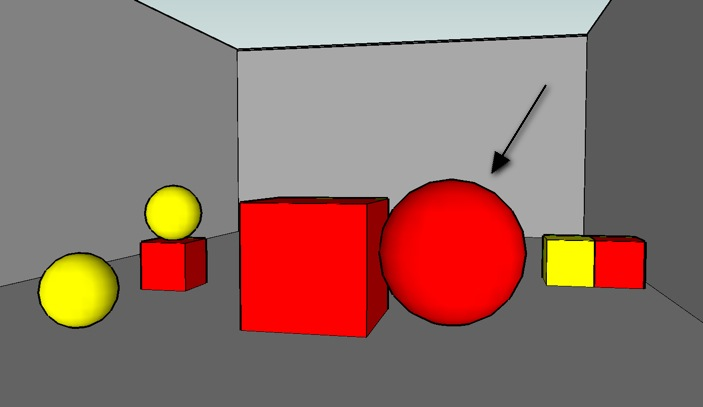
\includegraphics[width=0.6\textwidth]{images/22sinletras.jpg}
\caption{Ejemplo de contexto}
\label{GRE3D7-stimulus}
\end{figure}

Una propiedad es una caracter\'istica propia de un objeto. Por ejemplo en el Contexto \ref{GRE3D7-stimulus} el objeto se\~nalado con la flecha tiene la propiedad {\it color} con valor {\it rojo}. Por simplicidad, en el resto de la tesis vamos a decir ``tiene propiedad {\it rojo}'', cuando queremos decir que el objeto tiene la propiedad color con valor rojo. Una relaci\'on caracteriza a un objeto describiendo caracter\'isticas de otro u otros objetos.\\

%Cuando la ER no es relacional solo contiene propiedades del objeto mismo. Ej.: color, tama\~no. Note que quiz\'as el tama\~no sea con respecto a los dem\'as objetos ``la m\'as peque\~na'', pero al no incluir una descripci\'on de otro objeto no la llamamos relacional.\\
De acuerdo a las propiedades o relaciones que una expresi\'on referencial (ER) incluya, se clasifican en distintos tipos: relacional o no relacional (tambi\'en llamada proposicional), m\'inima, sobreespecificada, o subespecificada. A continuaci\'on describimos cada uno de estos tipos.\\

% en cuyo caso es una expresi\'on que no es referencial, la incluimos en nuestras propiedades porque nos va a ser \'util la definici\'on en el Cap\'itulo \ref{sec:corpus}.\\
Una ER {\it proposicional} o no relacional, incluye s\'olo propiedades intr\'insecas del objeto target. Por ejemplo en el Contexto \ref{GRE3D7-stimulus}: ``La esfera roja''. Las caracter\'isticas de ser esfera, ser roja son propias del objeto identificado.\\

Una ER es {\it relacional}, cuando adem\'as de ser proposicional, contiene relaciones con otros objetos, entonces la ER incluye las ERs de los otros objetos.  Por ejemplo en el Contexto \ref{GRE3D7-stimulus}: ``La esfera que esta a la derecha del cubo grande'', ``a la derecha de'' es una relaci\'on que necesita describir otro objeto adem\'as del target, en este caso ``el cubo grande''.\\

Se dice que una ER es {\it minimal}, cuando incluye la m\'inima cantidad de propiedades con las cuales el objeto puede ser distinguido en el contexto dado. Notar que puede haber muchas expresiones minimales. Por ejemplo en el Contexto \ref{GRE3D7-stimulus} ``La esfera roja'' es una ER minimal, como as\'i tambi\'en lo es ``La esfera grande'', ya que ambas tienen 2 propiedades, y 2 es la m\'inima cantidad de propiedades que puede tener una ER de ese objeto, para distinguirlo en ese contexto.\\

Cuando la ER contiene m\'as informaci\'on de la m\'inima necesaria para distinguirlo de los dem\'as objetos en el contexto dado, se dice que la ER es {\it sobreespecificada}. Por ejemplo: ``La esfera roja grande'' en el Contexto \ref{GRE3D7-stimulus}.\\

Una expresi\'on es {\it subespecificada} cuando no alcanza a ser una ER, ya que no se puede distinguir al objeto target de todos los objetos en el contexto. Por ejemplo: ``La esfera'' en el Contexto \ref{GRE3D7-stimulus} no alcanza para distinguir el objeto apuntado por la flecha, ya que hay otras 2 esferas. En estos casos se debe dar otra expresi\'on o corregir la anterior agregando m\'as propiedades o relaciones. Una expresi\'on subespecificada identifica a un conjunto, no a un objeto \'unico.

\section{La tarea de generaci\'on autom\'atica de expresiones referenciales}

La generaci\'on autom\'atica de expresiones referenciales (GER), es la tarea de definir cuales pasos se deben seguir para conseguir una ER de un objeto espec\'ifico, en un contexto dado. Estos pasos definen un algoritmo de GER. \\

Los algoritmos se pueden diferenciar por la cantidad y forma de los par\'ametros que toman como input, es decir el modo en que toman por ejemplo el contexto para el cual se espera que den una expresi\'on referencial. \\

En todos los casos, la computadora necesita tener un conjunto de propiedades/relaciones para cada objeto y poder identificarlos, para ello vamos a etiquetar a los objetos con $e_1$, $e_2$, etc. como se muestra en la Figura \ref{GRE3D7-stimulus-conLetras}. En la imagen tambi\'en podemos ver que el objeto se\~nalado con la flecha es $e_5$, es el objeto target, para el cual queremos generar autom\'aticamente una expresi\'on referencial.

\begin{figure}[ht]
\centering
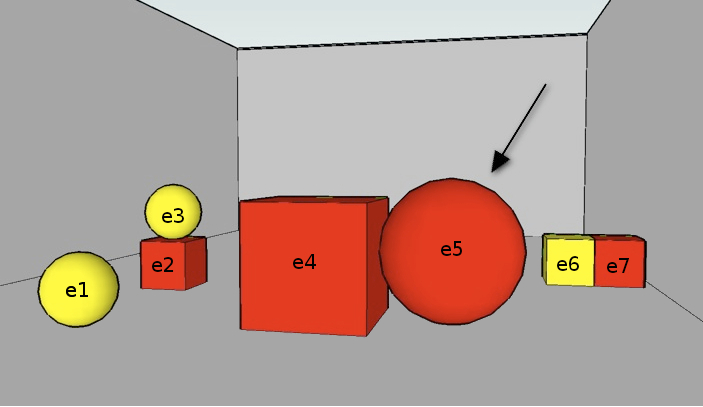
\includegraphics[width=0.6\textwidth]{images/22.jpg}
\caption{Ejemplo de contexto con objetos etiquetados}
\label{GRE3D7-stimulus-conLetras}
\end{figure}

A continuaci\'on daremos 2 ejemplos de diferentes maneras de modelar el contexto que toman como input, uno para el algoritmo Graph y otro para algoritmo de Bisimulaci\'on.\\

%El contexto que toma como input el algoritmo GRAPH \cite{graph08} el cual explicaremos en la Secci\'on \ref{graph}, para el Contexto \ref{GRE3D7-stimulus}, es un grafo dirigido y etiquetado como se muestra en Figura \ref{grafo-GRE3D7-stimulus}, el cual contiene la informaci\'on de las propiedades y relaciones de los objetos, por ejemplo podemos ver que el objeto target que es el $e_5$, tiene propiedades large, red, ball y una flecha con la etiqueta rightof $e_4$, y $e_4$ tiene propiedades large, red, cube, y una flecha hacia $e_5$ con etiqueta leftof.\\

El contexto que toma como input el algoritmo Graph \cite{graph08} el cual explicaremos en la Secci\'on \ref{graph}, para el Contexto \ref{GRE3D7-stimulus}, es un grafo dirigido y etiquetado como se muestra en Figura \ref{grafo-GRE3D7-stimulus}, el cual contiene la informaci\'on de las propiedades y relaciones de los objetos, por ejemplo podemos ver que el objeto $e_5$, tiene propiedades grande, rojo, esfera y una flecha con la etiqueta a-la-der-de hacia $e_4$, y $e_4$ tiene propiedades grande, rojo, cubo, y una flecha hacia $e_5$ con etiqueta a-la-izq-de.\\

Notaci\'on: a-la-der-de y a-la-izqu-de son relaciones las cuales significan ``a la derecha de'' y ``a la izquierda de'' respectivamente.\\

\begin{figure}[ht]
\centering
\begin{tikzpicture}
  [
    n/.style={circle,fill,draw,inner sep=3pt,node distance=2cm},
    aArrow/.style={->, >=stealth, semithick, shorten <= 1pt, shorten >= 1pt},
  ]
 \node[n,label=above:$e_1$,label=below:{
    \relsize{-2}$\begin{array}{c}
      \nSmall\\[-3pt] 
      \nYellow \\[-3pt] 
      \nBall\end{array}$}] (a) {};
 \node[n,label=above:$e_2$,label=below:{
    \relsize{-2}$\begin{array}{c}     
      \nSmall\\[-3pt] 
      \nRed\\[-3pt] 
      \nCube\end{array}$}, right of=a] (b) {};
 \node[n,label=below:$e_3$,label=above:{
    \relsize{-2}$\begin{array}{c}
      \nTop\\[-3pt]      
      \nSmall\\[-3pt] 
      \nYellow\\[-3pt] 
      \nBall\end{array}$}, above of=b] (c) {};
 \node[n,label=right:$e_4$,label=left:{
    \relsize{-2}$\begin{array}{c}
      \nLarge\\[-3pt] 
      \nRed\\[-3pt] 
      \nCube\end{array}$}, right of=b] (d) {};
 \node[n,label=left:$e_5$,label=below:{
    \relsize{-2}$\begin{array}{c}
      \nLarge\\[-3pt] 
      \nRed\\[-3pt] 
      \nBall\end{array}$}, right of=d] (e) {};
 \node[n,label=right:$e_6$,label=left:{
    \relsize{-2}$\begin{array}{c}
      \nSmall\\[-3pt] 
      \nYellow\\[-3pt] 
      \nCube\end{array}$}, right of=e] (f) {};
 \node[n,label=left:$e_7$,label=below:{
    \relsize{-2}$\begin{array}{c}
      \nSmall\\[-3pt]
      \nRed\\[-3pt] 
      \nCube\end{array}$},  right of=f] (g) {};
 \draw [aArrow,bend right=40] (b) to node[auto,swap]{\relsize{-3}$\nBelow$} (c);
 \draw [aArrow,bend right=40] (c) to node[auto,swap]{\relsize{-3}$\nOntop$} (b);
 \draw [aArrow,bend right=40] (d) to node[auto,swap]{\relsize{-3}$\nLeftof$} (e);
 \draw [aArrow,bend right=40] (e) to node[auto,swap]{\relsize{-3}$\nRightof$} (d);
 \draw [aArrow,bend right=40] (f) to node[auto,swap]{\relsize{-3}$\nLeftof$} (g);
 \draw [aArrow,bend right=40] (g) to node[auto,swap]{\relsize{-3}$\nRightof$} (f);
 \draw[dotted] (-0.5,-1.1) rectangle (10.5,3.1);

 \end{tikzpicture}
\caption{Grafo del contexto \ref{GRE3D7-stimulus}}
\label{grafo-GRE3D7-stimulus}
\end{figure}

Para el mismo Contexto \ref{GRE3D7-stimulus-conLetras}, el input del algoritmo de Bisimulaci\'on el cual explicaremos en Secci\'on \ref{bisimulacion}, es un archivo con formato XML \footnote{XML, siglas en ingl\'es de eXtensible Markup Language ('lenguaje de marcas extensible'), es un lenguaje de marcas desarrollado por el World Wide Web Consortium (W3C) utilizado para almacenar datos en forma legible.} con la misma informaci\'on del Contexto \ref{input-bisimulacion}. En este caso se representan las propiedades como relaciones a un objeto ficticio, terminal {\it c}, creado para modelar propiedades y relaciones, como relaciones, como veremos luego esto va a servir para dar prioridad a las relaciones en algunos casos. En el XML podemos ver que todos los objetos tienen ``id'' que es el identificador, salvo el objeto target $e_5$ el cual tiene {\it refer-to} en vez de {\it id}. Con la etiqueta ``rel'', identificamos las relaciones y con la etiqueta ``to'' con que objeto esta relacionado. En este ejemplo el target tiene relaciones con c (grande, rojo, esfera) y con $e_4$ a-la-derecha-de.  
%\'Este tiene las relaciones con c (large, red, ball) y con $e_4$ rightof.  
\textcolor{blue}{aca tengo problemas en verbatim para escribir la enie de pequeino}
\label{input-bisimulacion}

%\include{xml}

\begin{verbatim}
<?xml version="1.0"?>
<problem id="e1">c
  <individual id="e1">
    <related rel="pequeno" to="c" />
    <related rel="amarillo" to="c" />
    <related rel="esfera" to="c" />
  </individual>
  ...
  <individual id="e4">
    <related rel="cubo" to="c" />
    <related rel="rojo" to="c" />
    <related rel="grande" to="c" />
    <related rel="a-la-izq-de" to="e5" />
  </individual>
  <individual refer-to="e5">
    <related rel="grande" to="c"/>
    <related rel="esfera" to="c" />
    <related rel="rojo" to="c" />
    <related rel="a-la-der-de" to="e4" />
  </individual>
  ...
  <individual id="c">
    <related rel="terminal" to="c" />
  </individual> 
</problem>
\end{verbatim}
%\label{input-bisimulacion}
%\begin{verbatim}
%<?xml version="1.0"?>
%<problem id="e1">c
  %<individual id="e1">
    %<related rel="small" to="c" />
    %<related rel="yellow" to="c" />
    %<related rel="ball" to="c" />
  %</individual>
  %...
  %<individual id="e4">
    %<related rel="cube" to="c" />
    %<related rel="red" to="c" />
    %<related rel="large" to="c" />
    %<related rel="left-of" to="e5" />
  %</individual>
  %<individual refer-to="e5">
    %<related rel="large" to="c"/>
    %<related rel="ball" to="c" />
    %<related rel="red" to="c" />
    %<related rel="right-of" to="e4" />
  %</individual>
  %...
  %<individual id="c">
    %<related rel="terminal" to="c" />
  %</individual> 
%</problem>
%\end{verbatim}
%Saque para que no quede tan largo
%<individual id="e6">
    %<related rel="small" to="c" />
    %<related rel="cube" to="c" />
    %<related rel="yellow" to="c" />
    %<related rel="left-of" to="e7" />
  %</individual>
  %<individual id="e7">
    %<related rel="small" to="c" />
    %<related rel="cube" to="c" />
    %<related rel="red" to="c" />
    %<related rel="right-of" to="e6" />
  %</individual>

%<individual id="e2">
%    <related rel="cube" to="c" />
%    <related rel="red" to="c" />
%    <related rel="small" to="c" />
%    <related rel="bellow" to="e3" />
%  </individual>
%  <individual id="e3">
%    <related rel="ball" to="c" />
%    <related rel="yellow" to="c" />
%    <related rel="small" to="c" />
%    <related rel="on-top" to="e2" />
%  </individual>
Los algoritmos tambi\'en se pueden diferenciar por la clase de ER que pueden generar, a continuaci\'on explicaremos los distintos tipos de algoritmos de GER. 

\section{Tipos de algoritmos de GER}

Un algoritmo para la generaci\'on autom\'atica de expresiones referenciales  puede ser: determin\'{i}stico o no-determin\'{i}stico, relacional o proposicional, incluir negaciones o no, identificar plurales o s\'olo singulares,
 %usar disyunciones y conjunciones, o s\'olo conjunciones, 
generar ER sobreespecificadas o minimales.  A continuaci\'on se describen cada uno de esos tipos.\\

Un algoritmo es {\it determin\'{i}stico} si dado un input (un contexto y un objeto target), da siempre la misma ER de salida. En cambio un algoritmo es {\it no-determin\'{i}stico} si es posible que d\'e distintas salidas para el mismo input, en distintas ejecuciones. En general las personas generan expresiones referenciales de forma no determin\'istica, por lo tanto los algoritmos no determin\'isticos simulan el comportamiento de distintas personas, o incluso el de la misma persona en distintos momentos. Por ejemplo ser\'ia no determin\'istico si para el Contexto \ref{GRE3D7-stimulus-conLetras} una vez da ``La esfera roja'' y en otra ejecuci\'on ``La esfera grande''.\\

Un algoritmo es {\it proposicional}, cuando las ER que genera contienen solo atributos del target, es decir no contiene relaciones con otros atributos ni ER de otros objetos.  Por ejemplo para el Contexto \ref{GRE3D7-stimulus-conLetras} ``La esfera roja''.\\

Un algoritmo es {\it relacional} si adem\'as de generar ER proposicionales genera ER relacionales, en cuyo caso adem\'as de generar las relaciones correspondientes deber\'a generar ERs para el o los objetos relacionados. Por ejemplo para el Contexto \ref{GRE3D7-stimulus-conLetras} la ER ``La esfera roja a la derecha del cubo grande''. En este caso ``el cubo grande'' es una expresi\'on referencial que se tuvo que dar como consecuencia de incluir la relaci\'on ``a la derecha de''. En estos casos hay que asegurarse que el algoritmo termina, es decir que no entra en loops tratando de identificar objetos.\\

En algunos contextos cuando el target es el \'unico que no tiene una propiedad por ejemplo, ser\'ia \'util un algoritmo que incluya {\it negaciones}. Por ejemplo para el Contexto \ref{GRE3D7-stimulus-conLetras}, ``La \'unica esfera que no es peque\~na''.\\

Un algoritmo puede generar ER para {\it plurales}, es decir dar ER para varios targets en el contexto considerado. Por ejemplo para el Contexto \ref{plurales}, ``Los objetos grandes''. En este caso el target no es \'unico, sino un conjunto de objetos. \\

\begin{figure}[ht]
\centering
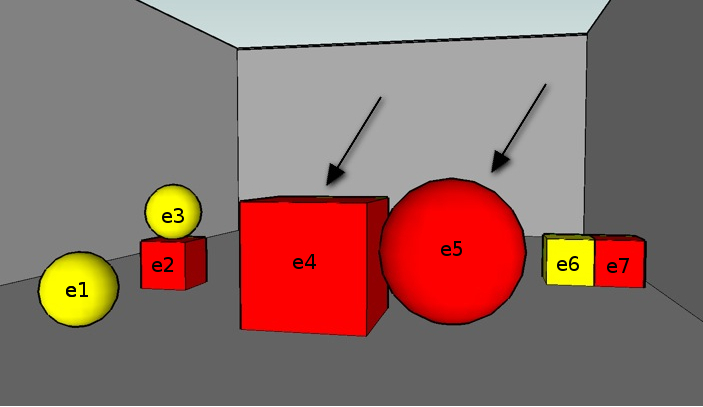
\includegraphics[width=0.6\textwidth]{images/22-plural.jpg}
\caption{Ejemplo de contexto con 2 targets}
\label{plurales}
\end{figure}
%esto lo saque porque confunde aca... me parece que todavia no hay que hablar de esto, es muy de logica
%Los algoritmos tambi\'en se pueden diferenciar en los conectores que permiten si usan conjunciones, disyunciones o ambas.\\

Un algoritmo que genera ER {\it minimales}, es un algoritmo que da ER que contienen la m\'inima cantidad de propiedades o relaciones que se necesitan para distinguir al target.  Por ejemplo para el Contexto \ref{GRE3D7-stimulus-conLetras} ``La esfera grande''. Notar que incluso puede haber varias ER minimales, como en este caso ``la esfera roja''.\\

Un algoritmo que genera ER {\it minimales}, es un algoritmo que da ER que contienen la m\'inima cantidad de propiedades o relaciones que se necesitan para distinguir al target.  Por ejemplo para el Contexto \ref{GRE3D7-stimulus-conLetras} ``La esfera grande''. Notar que incluso puede haber varias ER minimales, como en este caso ``la esfera roja''.\\

La {\it sobreespecificaci\'on} es la caracter\'istica de dar m\'as atributos o relaciones de las necesarias para identificar al objeto target. Por ejemplo para el Contexto \ref{GRE3D7-stimulus-conLetras} la ER ``La esfera roja, grande que esta a la derecha del cubo rojo grande'' es una ER sobreespecificada.\\

%no se si dejar esto...
%Un algoritmo que hace backtraking, es el que luego de incluir una propiedad o relaci\'on puede deshacer esa inclusi\'on volviendo a un estado anterior, es decir, decidir no incluirla.\\

\section{Algoritmos importantes en el \'area}
%interesante...
%https://www.abdn.ac.uk/ncs/departments/computing-science/tunabibl-495.php

En esta secci\'on vamos a hablar de los algoritmos de generaci\'on autom\'atica de expresiones referenciales, empezando por el algoritmo Full Brevity, el algoritmo de heur\'istica Greedy, siguiendo con el algoritmo Incremental, Graph, algoritmo Relacional y por \'ultimo Bisimulaci\'on.  \\

%http://citeseerx.ist.psu.edu/viewdoc/download?doi=10.1.1.227.8284&rep=rep1&type=pdf

%REG can be traced back to the earliest days of Natural Language Processing; Winograd
%(1972)  (Section  8.3.3,  Naming  Objects  and  Events),  for  example,  sketches  a  primitive
%“incremental” REG algorithm, used in his SHRDLU program. In the 1980s, researchers
%such as Appelt and Kronfeld set themselves the ambitious task of modelling the human
%capacity for producing and understanding referring expressions in programs such as
%KAMP and BERTRAND (Appelt 1985; Appelt and Kronfeld 1987; Kronfeld 1990). They
%argued that referring expressions should be studied as part of a larger speech act. KAMP
%(Appelt  1985),  for  example,  was  conceived  as  a  general  utterance  planning  system,
%building  on  Cohen  and  Levesque’s  (1985)  formal  speech  act  theory.

%REG  task  is  now  defined  by  Dale  and  Reiter  (1995)  through  what  may  be
%called identification of the target: given a target (or referent) object r 2 D , find a set of attribute–value  pairs L
%whose  conjunction  is  true  of  the  target  but  not  of  any  of  the
%distractors (i.e., D

%Full  Brevity  and  Greedy  Heuristic.
El algoritmo {\it Full Brevity} \cite{Dale:1989:CUR:981623.981632} genera la descripci\'on m\'as corta que identifica al target. Para hacerlo, 
busca si hay una propiedad del target que no sea propiedad de ning\'un distractor. Si no hay chequea todas las posibles combinaciones de 2 propiedades, si no la hay, busca de a 3 y as\'i sucesivamente.\\

El problema es que encontrar la descripci\'on m\'as corta es de alta complejidad, se observ\'o que las personas dan expresiones que no son minimales, esto fue confirmado por estudios psycoling\"uisticos (\cite{Olson1970LangAndThought};  \cite{Sonnenschein1984}; \cite{Pechmann1989}; \cite{Engelhardt2006}).\\

Una aproximaci\'on a Full Brevity es el algoritmo de heur\'istica {\it Greedy}, el cual iterativamente selecciona la propiedad que elimina m\'as distractores y argumentan que la propiedad seleccionada tiene el m\'as alto poder discriminativo en esa etapa. Como resultado no siempre genera expresiones referenciales m\'inimas.\\

%which  iteratively  selects  the  property  which  rules  out  most  of  the  distractors
%not  previously  ruled  out,  incrementally  augmenting  the  description  based  on  what
%property has most discriminatory power at each stage (as a result, it does not always
%generate  descriptions  of  minimal  size). 
El algoritmo de heur\'istica Greedy es m\'as eficiente que el Full Brevity, pero pronto fue superado por el algoritmo {\it Incremental} y sus sucesores \cite{C92-1038}; \cite{Dale95computationalinterpretations}. El algoritmo Incremental fue y sigue siendo uno de los algoritmos m\'as importantes del \'area, lo explicamos a continuaci\'on. 
% The  Greedy  Heuristic  algorithm  is  a  more
%efficient  algorithm  than  the  Full  Brevity  one,  but  it  was  soon  eclipsed  by  another
%algorithm    which  turned  out  to  be  the
%most influential algorithm of the pre-2000 era. It is this later algorithm that came to be
%known as``the'' Incremental Algorithm (IA).

%\subsection{GREEDY}

%El algoritmo GREEDY de Dale~\cite{dale89} busca sobre todo el conjunto de propiedades del target y elije el subconjunto m\'as chico posible que identifica un\'{i}vocamente al objeto target entre los distractores en la escena considerada como se muestra en el siguiente algoritmo.\\

%\begin{figure}[ht]
%\begin{center}
%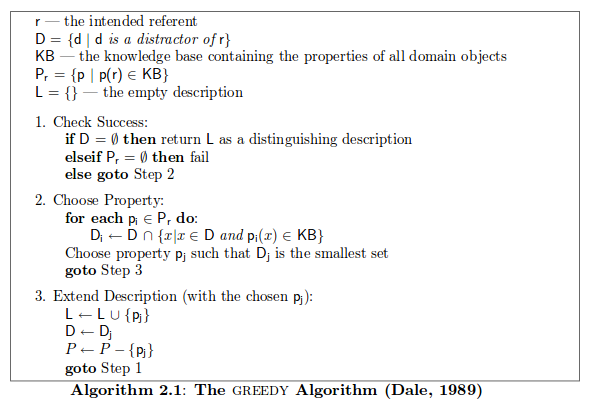
\includegraphics[width=8.5cm]{figures/greedy.png}\\[0pt]
%\caption{Interface del experimento}
%\label{fig-greedy}
%\end{center}
%\end{figure}

%r - el objeto target\\
%D = \{d|d es un distractor de r\}\\
%KB - la base de conocimiento que contiene las propiedades de todos los objetos\\
%$P_{r}$ = $\{p|p(r) \in KB\}$\\
%L = $\{\}$ - la descripci\'on vac\'{i}a\\
%\\
%1. Chequea \'exito:\\
%    \textbf{if} D = $\emptyset$ \textbf{then} return L como una ER que distingue al target r
%    \textbf{elseif} $P_{r}$ = $\emptyset$ \textbf{then} fail
%    
%\textbf{else goto} Paso 2 \\
%\\
%2. Elegir Propiedad:
% \textbf{for each} $p_{i}$ $\in$ $P_{r}$ \textbf{do}:
%    $D_{i}$ $\leftarrow$ D$\cap$ \{x|x $\in$ D and $p_{i}$ (x) $\in$ KB\}
%    Elegir la propiedad $p_{j}$ tal que $D_{j}$ es el conjunto m\'as chico (es decir la que elimina m\'as distractores) \textbf{goto} Paso 3\\
%\\    
%3. Agregar $p_{j}$ a la descripci\'on actual\\
%L $\leftarrow$ L $\cup$ \{$p_{j}$\}\\
%D $\leftarrow$ $D_{j}$\\
%P $\leftarrow$ P -\{$p_{j}$\}\\
%\textbf{goto} Paso 1\\



%%Dado un dominio D que contiene un target referente r y un conjunto de distractores, una base de conocimiento KB que contiene las propiedades de los objetos.
%%Un conjunto de propiedades verdaderas para r, y una descripcion L inicialmente vac\'{i}a.

%Este algoritmo es de orden NP-complete

\subsection{Incremental}

%A continuaci\'on se describe el algoritmo Incremental de Dale \& Reiter el cual esta basado en el algoritmo GREEDY (el cual hac\'ia una b\'usqueda exaustiva y eleg\'ia la propiedad que m\'as distractores eliminaba en cada paso) pero \'este reduce la complejidad del algoritmo Greedy cambiando que en vez de chequear cual propiedad es la que elimina m\'as distractores, eligiendo la que sigue en la lista de propiedades ordenada seg\'un preferencia y que elimina al menos un distractor. Este algoritmo es de orden polinomial. Este algoritmo produce expresiones referenciales que pueden estar sobreespecificadas.\\

\textcolor{blue}{error entorno matematico, pero no entiendo porque, y no puedo hacer que diga algoritmo en vez de algorithm}

%\begin{figure}
\small
\begin{center}
%\centering
\begin{algorithm}[H]

\dontprintsemicolon

\captionsetup[algorithm]{name=Algoritmo}
\caption{Incremental\label{algo:incremental}}
%\caption{Incremental}\label{algo:incremental}
\KwIn{\footnotesize \{r, D, Pref\} r es el target, D es el dominio, Pref lista de preferencia de propiedades ordenadas}
\KwOut{\footnotesize L  - Descripci\'on de salida}

$\ L \leftarrow \emptyset $ \tcp*[f]{\footnotesize Inicialmente es vac\'io}\\
$\ C \leftarrow D - \{r\} $ \tcp*[f]{\footnotesize C es el conjunto de todos los objetos menos r }\\


\For{\em $A_{i}$ $\in$ Pref }{
	$V = Value(r,A_{i})$ \tcp*[f]{\footnotesize V es el valor de la propiedad $A_{i}$ para r }\\
	\If(\tcp*[f]{\footnotesize Si elimina alg\'un distractor}){\em $C \cap RulesOut(\[A_{i}\],V) \neq \emptyset $}
	{
    $\ L \leftarrow L \cup \{A_{i},V\} $  \tcp*[f]{\footnotesize Agrega la propiedad $A_{i}$ a L }\\
    $\ C \leftarrow C - RulesOut(\[A_{i}\],V) $ \tcp*[f]{\footnotesize Actualiza C sacando los objetos que no tienen V en $A_{i}$} 
  }
  \If(\tcp*[f]{\footnotesize Si no quedan distractores}){\em $C = \emptyset$}
	{
     Return L 
  }
}
Return Fallo
\end{algorithm}
\end{center}
%\end{figure}



Como podemos ver en \ref{algo:incremental} el input de este algoritmo es el objeto target que queremos identificar {\it r}, D, el dominio, y Pref una lista ordenada de preferencia de propiedades.\\
En {\it Paso 1} se asigna a L la descripci\'on vac\'{i}a, al finalizar la ejecuci\'on, L tendr\'a el conjunto de propiedades con los cuales identificaremos a r, es decir una expresi\'on referencial de r. 
Se le asigna a C el conjunto de distractores de r (todos los objetos menos r), en {\it Paso 2}.\\

La idea del algoritmo es ir eliminando distractores, por eso, en el {\it Paso 3} recorre las propiedades de r. En {\it Paso 4} le asigna a V el valor que tiene el target para la propiedad $A_{i}$

$RulesOut(A_{i},V)$ devuelve el conjunto de objetos que tienen diferente valor para la propiedad $A_{i}$ que el que tiene el objeto target.

Si hay objetos en C que tengan diferente valor de $A_{i}$ que el target, se agrega la propiedad a la descripci\'on actual L en {\it Paso 6}, y se actualiza $C$ sacando los objetos que no tienen V en $A_{i}$. 

Luego en {\it Paso 8} si C es $\emptyset$ (si no hay m\'as distractores) devolvemos L, como el conjunto de propiedades que identifican a r.

Vamos a ejemplificar la corrida del algoritmo con el ejemplo de Contexto \ref{GRE3D7-stimulus-conLetras}, y supongamos que la lista ordenada de propiedades es esta [ tipo, color, tama\~no ]. D inicialmente es \{$e_{1}$,$e_{2}$,$e_{3}$,$e_{4}$,$e_{5}$,$e_{6}$,$e_{7}$\}
Al iniciar a L le asigna $\emptyset$ y a C \{$e_{1}$,$e_{2}$,$e_{3}$,$e_{4}$,$e_{6}$,$e_{7}$\}, luego comienza a recorrer la lista de propiedades, la primer propiedad es ``tipo'', el valor del target para tipo es {\it esfera}, entonces en {\it Paso 6}, pregunta si hay objetos que tengan tipo con valor distinto de esfera, y hay, ellos son \{$e_{2}$,$e_{4}$,$e_{6}$,$e_{7}$\}, entonces le asigna a C \{$e_{1}$,$e_{3}$\}, es decir solo las esferas. En {\it Paso 10} pregunta si C es vac\'io, no lo es, por lo tanto continua con la siguiente propiedad, en este caso ``color'', el valor de color para el target es {\it rojo}, agrega {\it rojo} a L, y actualiza C con $\emptyset$ porque tanto $e_{1}$ como $e_{3}$ son amarillos, en {\it Paso 10} pregunta si C es vac\'io, y si lo es, por lo tanto devuelve \{esfera, rojo\}.


%Intuitivamente, si la primer propiedad tipo y el valor de tipo para el target es ``esfera'', nos quedamos con todos los objetos esfera.\\

%\textcolor{blue}{Un poco mas de historia, no se a donde poner...Theune and Krahmer proposed an extension that allows the generation of subsequent reference with the ia taking into account the discourse salience of the target referent (Krahmer and Theune, 1998; Theune, 2000; Krahmer and Theune, 2002), and a second one which allows the ia to produce referring expressions that
%contain binary relations to other objects (Theune, 2000; Krahmer and Theune, 2002). I will return to their relational extension in Section 2.3. Theune and Krahmer's approach works by assigning a salience score to all objects according to the
%focus/topic distinction by Hajicova (1993) and Centering Theory (Grosz et al., 1995). They alter the success criterion of the algorithm and only let it stop when here is no distractor left that is as or more salient than the target referent.
%Not all properties are the same. The qualitative diferences that exist between diferent properties were first discussed in the
%reg literature by van Deemter (2000, 2006). He pointed out that the appropriateness of
%vague orgradable properties such as small and large is dependent on the context in which they are used, while,
%for example, the colour of an object is absolute. Consider two descriptions in a domain of animals... (van Deemter, 2002), van Deemter considered the ia's logical completeness in terms of the Boolean operators of negation and disjunction. He extended it to
%be able to generate referring expressions that contain negated properties, such as Example (2.3), and descriptions of sets of objects, such as Example (2.4), or even (2.5), which contains a logical disjunction of properties. His algorithm proceeds
%in stages, trying longer and longer disjunctions of properties, if atomic properties
%and shorter disjunctions did not suffice to distinguish the target set.. he work on reference to sets was taken further by Gatt and van Deemter (2005, 2006), who have presented the most mature algorithms in this space to
%date. They used a similar procedure to the ia in that their algorithms are based
%on incremental processing of a preference order of properties. Their algorithms
%add a lot of complex machinery to the basic procedure to ensure that properties
%are chosen in a way that maximises coherence within the set of objects described
%by the referring expressions. For example, their approach will attempt to use
%properties of the same type for all the referents of a set. So, it would produce
%descriptions such as Examples 
Luego se propusieron extensiones del algoritmo Incremental, por ejemplo 
Theune y Krahmer propusieron una extensi\'on que permite la generaci\'on de referencia teniendo en cuenta la prominencia discurso del target (\cite{Krahmer:2010:EMN:1880370}; \cite{krahmer-theune:2002a};), y un segundo algoritmo que permite producir expresiones referenciales que contienen relaciones con otros objetos. El enfoque Theune y de Krahmer funciona asignando una puntuaci\'on de relevancia a todos los objetos de acuerdo con el enfoque / tema distinci\'on por \cite{hajicova-1993} y la teor\'ia de centrado \cite{Grosz:1995:CFM:211190.211198}. Alteran el criterio de \'exito del algoritmo y s\'olo permiten que se detenga cuando hay un distractor que es tanto o m\'as relevante que el target.
No todas las propiedades tienen la misma relevancia. Las diferencias cualitativas que existen entre diferentes propiedades se discutieron por primera vez en la literatura GER por van Deemter (2000, 2006). Se\~nal\'o que la conveniencia de otras propiedades sobre las
propiedades vagas como peque\~no y grande dependen del contexto en el que se utilizan, mientras que, por ejemplo, el color de un objeto es absoluta. 
%Considere dos descripciones de un dominio de los animales ... (van Deemter, 2002), van Deemter considera integridad l\'ogica del ia en t\'erminos de los operadores booleanos de negaci\'on y disyunci\'on. \'el la extendi\'o a
%ser capaz de generar expresiones referenciales que contienen propiedades, tales como Ejemplo (2.3) negado, y las descripciones de conjuntos de objetos, tales como Ejemplo (2.4), o incluso (2,5), que contiene una disyunci\'on l\'ogica de propiedades. Sus algoritmo procede
%en etapas, tratando m\'as y disyunciones m\'as largos de propiedades, si las propiedades at\'omicas
%y disyunciones m\'as cortos no son suficientes para distinguir el conjunto target .. que funciona en referencia a conjuntos fue tomada adem\'as por Gatt y van Deemter (2005, 2006), que han presentado los algoritmos m\'as maduros a la fecha. Utilizaron un procedimiento similar al de las otras cosas en que sus algoritmos se basan en el procesamiento incremental de un orden de preferencia de las propiedades. Sus algoritmos agregan una gran cantidad de maquinaria compleja para el procedimiento b\'asico para asegurar que las propiedades
%se eligen de manera que maximiza la coherencia dentro del conjunto de objetos descritos por las expresiones referenciales. Por ejemplo, su enfoque intentar\'a utilizar propiedades del mismo tipo para todos los referentes de un conjunto. As\'i, ser\'ia producir
%descripciones tales como ejemplos
%(2.6) or (2.7) rather than Example (2.8) or.. 


%Theune y Krahmer propusieron una extensi\'on que permite la generaci\'on de referencia con la subsiguiente ia teniendo en cuenta la prominencia discurso del referente objetivo (Krahmer y Theune, 1998; Theune, 2000; Krahmer y Theune, 2002), y un segundo uno que permite la IA para producir expresiones referenciales que contener relaciones binarias a otros objetos (Theune, 2000; Krahmer y Theune, 2002). Voy a volver a su extensi\'on relacional en la Secci\'on 2.3. Enfoque Theune y de Krahmer funciona asignando una puntuaci\'on de relevancia a todos los objetos de acuerdo con la enfoque / tema distinci\'on por Hajicova (1993) y el centrado Theory (Grosz et al., 1995). Alteran el criterio de \'exito del algoritmo y s\'olo permiten que se detenga cuando aqu\'i hay izquierda distractor que es tan o m\'as relevante que el referente de destino.
%No todas las propiedades son las mismas. Las Diferencias cualitativas que existen entre diferentes propiedades se discutieron por primera vez en la literatura reg por van Deemter (2000, 2006). Se\~nal\'o que la conveniencia de propiedades orgradable vagos como peque\~nos y grandes depende del contexto en el que se utilizan, mientras que, Por ejemplo, el color de un objeto es absoluta. Considere dos descripciones de un dominio de los animales ... (van Deemter, 2002), van Deemter considera integridad l\'ogica del ia en t\'erminos de los operadores booleanos de negaci\'on y disyunci\'on. \'el la extendi\'o a ser capaz de generar expresiones que se refieren que contienen propiedades, tales como Ejemplo (2.3) negado, y las descripciones de conjuntos de objetos, tales como Ejemplo (2.4), o incluso (2,5), que contiene una disyunci\'on l\'ogica de propiedades. Sus algoritmo procede en etapas, tratando m\'as y disyunciones m\'as largos de propiedades, si las propiedades at\'omicas y disyunciones m\'as cortos no son suficientes para distinguir el conjunto de destino .. que funciona en referencia a conjuntos fue tomada adem\'as por Gatt y van Deemter (2005, 2006), que han presentado los algoritmos m\'as maduros en este espacio para la fecha. Utilizaron un procedimiento similar al de las otras cosas en que sus algoritmos se basan en el procesamiento incremental de un orden de preferencia de las propiedades. Sus algoritmos agregar una gran cantidad de maquinaria compleja para el procedimiento b\'asico para asegurar que las propiedades se eligen de manera que maximiza la coherencia dentro del conjunto de objetos descritos por las expresiones que se refieren. Por ejemplo, su enfoque intentar\'a utilizar propiedades del mismo tipo para todos los referentes de un conjunto. As\'i, ser\'ia producir Ejemplos descripciones tales como (2,6) o (2,7) en lugar de Ejemplo (2.8) o ..


\subsection{Algoritmo de b\'usqueda en Grafo}
\label{graph}
%Un grafo es un conjunto de objetos llamados v\'ertices o nodos unidos por enlaces llamadas aristas o arcos, que permiten representar relaciones binarias entre elementos de un conjunto. \\

Un grafo G es un par ordenado $G=(V,E)$, donde:
\begin{itemize}
   \item V es un conjunto de v\'ertices o nodos, y
    \item E es un conjunto de aristas o arcos, que relacionan estos nodos.

%\item Se llama orden del grafo G a su n\'umero de v\'ertices, $|V|$.

%\item El grado de un v\'ertice o nodo $v \in V$ es igual al n\'umero de arcos que lo tienen como extremo.

%\item Un bucle es una arista que relaciona al mismo nodo; es decir, una arista donde el nodo inicial y el nodo final coinciden.

%\item Dos o m\'as aristas son paralelas si relacionan el mismo par de v\'ertices.

%\item Un grafo puede ser dirigido o no, etiquetado o no.
\end{itemize}
%T\'{i}picamente, un grafo se representa gr\'aficamente como un conjunto de puntos (v\'ertices o nodos) unidos por l\'{i}neas (aristas).

Los grafos han sido muy estudiados, pr\'acticamente cualquier problema puede ser expresado como un problema de grafos, y aplicar algoritmos de b\'usqueda ya estudiados.

El algoritmo Graph de \cite{Krahmer:2003} propone ver la obtenci\'on de expresiones referenciales como un problema de grafos, el contexto que incluye al target y los distractores es representado como un grafo. \\

Cada objeto de la escena se modela como un v\'ertice en el grafo. Las propiedades at\'omicas como color, tipo o tama\~no se representan como un bucle en el correspondiente nodo. Est\'an etiquetados con los nombres de las propiedades y los valores que el objeto en cuesti\'on tiene para estas propiedades. \\

Las relaciones binarias entre objetos, por ejemplo abajo-de, arriba-de se modelan como aristas entre los nodos correspondientes.\\

%La base de conocimiento que incluye al target ahora esta expresada como los v\'ertices, las aristas y las etiquetas del grafo.\\

%Krahmer et al.'s (2003) reformularon la tarea de seleccionar las propiedades y relaciones que contendr\'a una expresi\'on referencial como un problema de teor\'ia de grafos.

Para generar una descripci\'on distintiva, el algoritmo busca un subgrafo del grafo original que identifica al target un\'{i}vocamente, le llama grafo distintivo.\\% (distinguishing graph).\\

Comenzando con el subgrafo que contiene un solo v\'ertice, que representa al target, se realiza una b\'usqueda exhaustiva, pero comenzando a lo ancho. Utiliza una heur\'{i}stica basada en el costo (costo de incluir propiedades, relaciones) para podar el espacio de b\'usqueda. Y da el grafo de menor costo. \\


%esto no se entiende nada
%Informalmente, un subgrafo refiere al target si y s\'olo si puede ser
%`Colocado sobre el gr\'afico de dominio de tal manera que el v\'ertice que representa subgrafo
%del objeto target se puede `coloca sobre 'el v\'ertice del objetivo en el gr\'afico de dominio,
%y cada uno de los bordes marcados en el subgrafo puede ser `coloca sobre 'un correspondiente
%borde en el gr\'afico de dominio con la misma etiqueta y el mismo sentido. Por otra parte,
%un subgrafo distingue al target un\'ivocamente si y s\'olo si se puede `colocarlo sobre grafo original' y es exactamente el
%v\'ertice target. La noci\'on informal de un gr\'afico que se coloca sobre otro corresponde al concepto te\'orico matem\'atico de isomorfismo de grafos.

En teor\'{i}a de grafos, un isomorfismo entre dos grafos G y H es una biyecci\'on f entre los conjuntos de sus v\'ertices $f:V(G) \rightarrow V(H)$ que preserva la relaci\'on de adyacencia. Es decir, cualquier par de v\'ertices u y v de G son adyacentes si y solo si lo son sus im\'agenes, $f(u)$ y $f(v)$, en H.\\

%\textcolor{blue}{aca quiero poner un ejemplo que muestre una imagen y el modelo como grafo}

La funci\'on de costo esta definida sobre las aristas y v\'ertices del grafo dominio. El costo de un subgrafo se define como la suma sobre todas las aristas y v\'ertices que contiene el grafo.\\
El algoritmo de b\'usqueda garantiza encontrar el subgrafo de menor costo que representa al target.\\

La funci\'on de costo es usada para podar las ramas del \'arbol de b\'usqueda cuando estas se hacen m\'as costosas que el grafo de menor costo encontrado hasta el momento. Esta funci\'on hace que se prefieran propiedades sobre otras que tienen mayor costo.

Por ejemplo, 
Los algoritmos discutidos por Dale y Reiter (1995) pueden ser vistos como
diferentes instancias de un algoritmo de b\'usqueda (Bohnet y Dale 2005; Gatt de 2007).
Todos ellos, b\'asicamente, buscan a trav\'es de un mismo espacio de estados, compuestos por tres componentes: conjunto de cosas verdaderas para el target, un conjunto de distractores, y un conjunto de propiedades del target que a\'un no han sido consideradas. El estado inicial se puede formalizar como la tripla ($\emptyset$, C, P) 
(no hay descripci\'on del target constru\'ida, no se han descartado distractores, y todas las propiedades P del target todav\'ia est\'an disponibles), y el estado final como
(L, $\emptyset$, P'), se ha encontrado una descripci\'on que distingue al target,
el conjunto de distractores est\'a vac\'io, y pueden o no quedar propiedades del target en P'. Todos los otros estados en el espacio de b\'usqueda son intermedios,
a trav\'es de cuales un algoritmo podr\'ia moverse en funci\'on de su estrategia de b\'usqueda. 
Por ejemplo 
cuando buscamos de una descripci\'on distintiva de $e_{5}$ del Contexto\ref{GRE3D7-stimulus-conLetras}, un estado intermedio podr\'ia ser
s = ({[forma, esfera],[color,rojo]},{$e_{5}$}, {[taman\~o, grande],[a-la-der-de, $e_4$]})

Los algoritmos discutidos anteriormente difieren en el m\'etodo de creaci\'on de los estados, y en el orden en que estos estados son recorridos. Full Brevity, por ejemplo, utiliza un m\'etodo de expansi\'on, que crea un nuevo estado para cada atributo
del target no contemplado antes (y que excluye al menos un distractor). 


Comenzando desde el estado inicial y aplicando a nuestro ejemplo de contexto, este m\'etodo ser\'ia dar\'ia lugar a tres nuevos estados, la creaci\'on de descripciones, incluyendo la informaci\'on de forma, el color, y el taman\~o, respectivamente. Estos estados son chequeados mediante un m\'etodo de amplitud-primero. 
El IA, por el contrario, utiliza un m\'etodo diferente para ampliar el grafo, cada vez que crea
un nuevo estado, lo hace de acuerdo con un orden de preferencia predeterminado. As\'i, en
el estado inicial, y suponiendo que (como antes) que escribe es el atributo m\'as preferido, el
ampliar m\'etodo ser\'ia crear un solo nuevo estado: s = {[forma, esfera]}, siempre hay 1 solo nuevo estado elegido por el orden de preferencia.



\subsection{Bisimulaci\'on}
\label{bisimulacion}

%Este algoritmo fue propuesto por %\cite{}

La idea es transformar el problema de GER al problema de computar una f\'ormula de l\'ogicas para la descripci\'on (DL) cuya extensi\'on sea el elemento target (o los elementos targets, en el caso de querer dar una ER para plurales aprovechando que una f\'ormula describe un conjunto que puede contener m\'as de un elemento).\\

A continuaci\'on daremos una introducci\'on a las l\'ogicas para la descripci\'on \alc y \el.\\

\emph{F\'ormulas} (o \emph{conceptos}) $\varphi$ de $\alc$ son generadas por la siguiente gram\'atica:
$$
\varphi,\varphi' ::= \top \mid p \mid \neg \varphi \mid \varphi \sqcap \varphi'
\mid \exists R. \varphi
$$
donde $p$ es el conjunto de los s\'imbolos proposicionales \prop y $R$ es el de los s\'imbolos relacionales \rel. $\el$ es la parte sin negaci\'on de $\alc$.\\

Las f\'ormulas de ambos $\alc$ y $\el$ son interpretadas en modelos relacionales de primer orden $\gM = (\Delta,\interp{\cdot})$ donde
$\Delta$ es un conjunto no vac\'io y $\interp{\cdot}$ es una funci\'on de interpretaci\'on tal que:
$$
\begin{array}{ccl}
\interp{p} & \subseteq & \Delta  \mbox{ para $p \in \prop$}\\
\interp{R} & \subseteq & \Delta \times \Delta  \mbox{ para $R \in \rel$}\\
\interp{\neg \varphi} & = & \Delta - \interp{\varphi}\\
\interp{\varphi \sqcap \varphi'} & = & \interp{\varphi} \cap \interp{\varphi'}\\
\interp{\exists R.\varphi} & = & \{i \mid \mbox{para alg\'un } i', (i,i') \in \interp{R}\\
& & \mbox{ e } i' \in \interp{\varphi} \}.\\
\end{array}
$$

\begin{figure}[ht]
\begin{center}
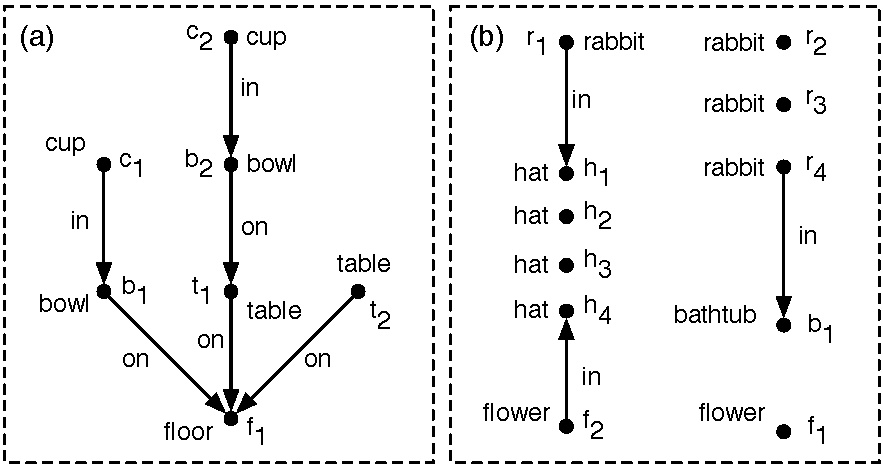
\includegraphics[width=8.5cm]{figures/pic-dale-haddock.pdf}\\[0pt]
\caption{}
\label{fig:dale-haddock}
\end{center}
\end{figure}


Cada f\'ormula de una descripci\'on l\'ogica denota un conjunto de objetos del dominio; por lo tanto podemos usar tales f\'ormulas para describir conjuntos. Por ejemplo en el modelo de la Figura.~\ref{fig:dale-haddock}b, la f\'ormula
$\mathsf{flower}$ denota el conjunto $\{f_1,f_2\}$; La f\'ormula
$\mathsf{flower} \sqcap \exists \mathsf{in}.\mathsf{hat}$ denota
$\{f_2\}$; y la f\'ormula $\mathsf{flower} \sqcap \neg
\exists \mathsf{in}.\mathsf{hat}$ denota $\{f_1\}$.\\

\textcolor{blue}{no se si dejar este ejemplo, o cambiarlo por uno es espa\~nol}

Hay muchas otras l\'ogicas de descripci\'on (DL) en la literatura por ejemplo 

$\mathcal{CL}$ (\el\ sin el cuantificador existencial, es decir solo conjunciones at\'omicas); $\mathcal{PL}$ (\alc\ l\'ogica propocisional); y
$\mathcal{ELU}_{(\neg)}$ (\el\ m\'as disjunci\'on y negaci\'on at\'omica).\\

Usaremos una noci\'on de preservaci\'on de f\'ormulas que llamaremos
\emph{similaridad}. Para cualquier DL $\gL$, diremos que un individual $i$ es \emph{\gL-similar} a $i'$ en un modelo dado $\gM$
si para cualquier f\'ormula $\varphi \in \gL$ tal que $i \in
\interp{\varphi}$, tambi\'en tenemos que $i' \in \interp{\varphi}$.\\
Equivalentemente, no hay $\gL$-f\'ormula que se mantenga para $i$ pero no para
$i'$.  Diremos que el \emph{\gL-conjunto de similaridad} de alg\'un individual
$i$ es el conjunto de todos los individuales a los cuales $i$ es \gL-similar.\\

Notar que la similaridad no es necesariamente una relaci\'on sim\'etrica: Por ejemplo:$f_1$ es \el-similar a $f_2$ en
Figura~\ref{fig:dale-haddock}b, pero $f_2$ no es \el-similar a $f_1$
(satisface la f\'ormula $\exists \mathsf{in}.\mathsf{hat}$ y $f_1$
no la satisface).  De todas maneras, \alc-similaridad es una relaci\'on sim\'etrica porque
el languaje contiene negaci\'on; y en consecuencia, $f_1$ no es \alc-similar
a $f_2$ porque este tampoco satisface $\neg \exists
\mathsf{in}.\mathsf{hat}$.  Porque \alc\ es m\'as expresivo que \el,
esto es, para alg\'un individual $a$ es posible ser \el-similar pero
no \alc-similar a alg\'un individual $b$, pero no viceversa.\\



%\textcolor{blue}{SACAR ESTO... poner quizas en la introduccion o en primer capitulo. Las ER que involucran relaciones han recibido m\'as atenci\'on recientemente;
%especialmente en el contexto de las expresiones referenciales espaciales en generaci\'on (por ejemplo,~\cite{kelleher06:increm}), donde es particularmente natural utilizar expresiones que implican relaciones espaciales, tales como ``la esfera en la parte superior del cubo''. Sin embargo, el algoritmo cl\'asico por~\cite{dale91:gener} ha demostrado ser incapaz de generar ER satisfactorias en la pr\'actica (v\'ease el an\'alisis sobre el~\emph{cabinet corpus} en~\cite{viethen06:_algor_for_gener_refer_expres}). Adem\'as, el Dale y Haddock algoritmo y muchos de sus sucesores (tales como~\cite{kelleher06:increm}) son vulnerables a el problema de la \emph{regresi\'on infinita}, donde el algoritmo entra en un bucle infinito, saltando hacia atr\'as y hacia adelante entre las descripciones para dos individuos emparentados, como en `` el libro sobre la mesa que soporta una libro sobre la mesa \ldots ''}

%REs involving relations have received increasing attention recently;
%especially in the context of spatial referring expressions in situated
%generation (e.g., \cite{kelleher06:increm}),
%where it is particularly natural to use expressions involving spatial
%relations such as ``the ball on top of the cube.''  However, the
%classical algorithm
%by~\cite{dale91:gener} was shown to be
%unable to generate satisfying REs in practice (see the analysis over
%the \emph{cabinet corpus}
%in~\cite{viethen06:_algor_for_gener_refer_expres}).  Furthermore, the
%Dale and Haddock algorithm and many of its successors (such
%as~\cite{kelleher06:increm}) are vulnerable to
%the problem of \emph{infinite regress}, where the algorithm enters an
%infinite loop, jumping back and forth between descriptions for two
%related individuals, as in ``the book on the table which supports a
%book on the table \ldots''

%\cite{arec2:2008:Areces,arec:usin11} have proposed low complexity
%algorithms for the generation of relational REs
%%(including references to sets) 
%that eliminate the risk of infinite regression.  These algorithms are
%based on variations of the partition refinement algorithms
%of~\cite{paig:thre87}.  The information provided by a given scene
%is interpreted as a relational model whose objects are classified into
%sets that fit the same description.  This classification is
%successively \emph{refined} till the target is the only element
%fitting the description of its class.  The existence of an ER depends
%on the information available in the input scene, and on the expressive
%power of the formal language used to describe elements of the
%different classes in the refinement.


\cite{arec2:2008:Areces,arec:usin11} han propuesto algoritmos de baja complejidad
 para la generaci\'on de ER relacionales que eliminan el riesgo de regresi\'on infinita. Estos algoritmos son
basados en variaciones de los algoritmos de refinamiento de particiones
de~\cite{paig:thre87}. La informaci\'on proporcionada por una escena dada
se interpreta como un modelo relacional cuyos objetos se clasifican en
conjuntos que se adaptan a la misma descripci\'on. Esta clasificaci\'on es
sucesivamente \emph{refinada} hasta que el target es el \'unico elemento
en la clase. La existencia de una ER depende
de la informaci\'on disponible en la escena de entrada, y del poder expresivo
del lenguaje formal utilizado para describir los elementos de las
diferentes clases en el refinamiento.\\

%Refinement
%algorithms %presented in~\cite{arec2:2008:Areces,arec:usin11}
%effectively compute REs for all individuals in the domain, at the same
%time. The algorithms always terminate returning a formula of the
%formal language chosen that uniquely describes the target (if the
%formal language is expressive enough to identify the target in the
%input model).
%\cite{arec2:2008:Areces}
%show that the refinement algorithm using the description language \el  is capable of generating 67\% of 
%the relational REs in the~\cite{viethen06:_algor_for_gener_refer_expres} dataset, when all possible orders of the relations in the domain are considered. This is in sharp contrast with the analysis 
%done in~\cite{viethen06:_algor_for_gener_refer_expres} over the cabinet corpus, of algorithms based in Dale and Reiter's original proposal.    

%Los algoritmos de refinamiento
% presenta en~\cite{arec 2:2008:Areces, arec:usin11}
%calculan efectivamente ER para todos los objetos en el dominio, al mismo
%tiempo. Los algoritmos siempre terminan devolviendo una f\'ormula del
%lenguaje formal elegido que describe un\'{i}vocamente el target (si el
%lenguaje formal es suficientemente expresivo para identificar el target en el
%modelo de entrada).\\

%Refinement algorithms for GER are based on the following basic idea:
%given a scene $S$, the objects appearing in $S$ are successively
%classified according to their properties into finer and finer
%classes. A description (in some formal language $\mathcal{L}$) of each
%class is computed every time a class is refined. The procedure always
%stops when the set of classes stabilizes, i.e., no further refinement
%is possible with the information available in the scene\footnote{Of
%  course, if we are only interested in a referring expression for a
%  given target we can stop the procedure as soon as the target is the
%  only element of some of the classes.}.  If the target element is in
%a singleton class, then the formal description of that class is a
%referring expression; otherwise the target cannot be unequivocally
%described (in 


%It is clear that a scene can be encoded in different ways as a
%relational model (for example in \ref{figure22}, we could argue that
%$e_1$ is also \emph{leftof} $e_2$, not considered because they are no
%touching). The algorithm assumes that these issues have been resolved
%and that the model encodes a suitable representation of the scene we
%want to describe.  Moreover, we will assume that all relations are
%\emph{binary}.  We will not consider relations of arity greater than
%two (relations of higher arity can be encoded as binary relations via
%reification, if necessary).

\begin{figure}[ht]
%\begin{minipage}[b]{0.45\linewidth}
%\centering
\begin{center}
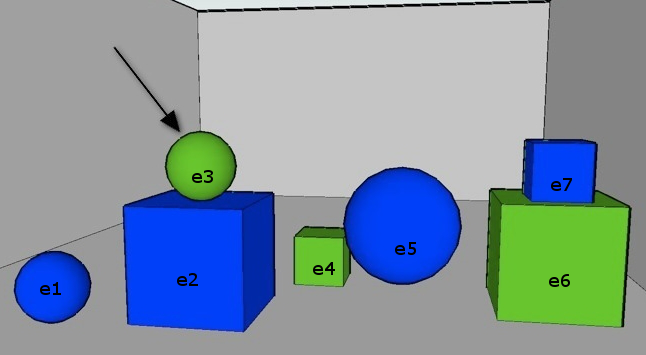
\includegraphics[width=0.5\textwidth]{images/3b.png}
\caption{Contexto de ejemplo}\label{GRE3D7-stimulus-cap2}
%\end{minipage}
\end{center}
\end{figure}

%\textcolor{blue}{hice mas grande la figura porque no se leian, como la pase a espaniol y se me fue al pie, no se porque}
%\hspace*{-0.35cm}
\begin{figure}[ht]
\begin{center}
%\begin{minipage}[b]{0.5\linewidth}
%\centering
\begin{tikzpicture}
  [
    n/.style={circle,fill,draw,inner sep=3pt,node distance=2.6cm},
    aArrow/.style={->, >=stealth, semithick, shorten <= 2pt, shorten >= 2pt},
  ]
 \node[n,label=above:$e_1$,label=below:{
    \relsize{-1}$\begin{array}{c}
      \nLeft\\[-2pt]
      \nSmall\\[-2pt] 
      \nBlue \\[-2pt] 
      \nBall\end{array}$}] (a) {};

 \node[n,label=above:$e_2$,label=below:{
    \relsize{-1}$\begin{array}{c}
      \nLeft\\[-2pt]
      \nBig\\[-2pt] 
      \nBlue\\[-2pt] 
      \nCube\end{array}$}, right of=a] (b) {};

 \node[n,label=below:$e_3$,label=above:{
    \relsize{-1}$\begin{array}{c}
      \nTop\\[-2pt]
      \nLeft\\[-2pt]
      \nSmall\\[-2pt] 
      \nGreen\\[-2pt] 
      \nBall\end{array}$}, above of=b] (c) {};

 \node[n,label=above:$e_4$,label=below:{
    \relsize{-1}$\begin{array}{c}
      \nSmall\\[-2pt] 
      \nGreen\\[-2pt] 
      \nCube\end{array}$}, right of=b] (d) {};

 \node[n,label=above:$e_5$,label=below:{
    \relsize{-1}$\begin{array}{c}
      \nBig\\[-2pt] 
      \nBlue\\[-2pt] 
      \nBall\end{array}$}, right of=d] (e) {};

 \node[n,label=above:$e_6$,label=below:{
    \relsize{-1}$\begin{array}{c}
      \nBig\\[-2pt] 
      \nGreen\\[-2pt] 
      \nCube\end{array}$}, right of=e] (f) {};

 \node[n,label=below:$e_7$,label=above:{
    \relsize{-1}$\begin{array}{c}
      \nTop\\[-2pt]
      \nSmall\\[-2pt] 
      \nBlue\\[-2pt] 
      \nCube\end{array}$}, above of=f] (g) {};

 \draw [aArrow,bend right=90] (b) to node[auto,swap]{\relsize{-1}$\nBelow$} (c);
 \draw [aArrow,bend right=90] (c) to node[auto,swap]{\relsize{-1}$\nOntop$} (b);

 \draw [aArrow,bend right=70] (d) to node[auto,swap]{\relsize{-1}$\nLeftof$} (e);
 \draw [aArrow,bend right=70] (e) to node[auto,swap]{\relsize{-1}$\nRightof$} (d);

 \draw [aArrow,bend right=90] (f) to node[auto,swap]{\relsize{-1}$\nBelow$} (g);
 \draw [aArrow,bend right=90] (g) to node[auto,swap]{\relsize{-1}$\nOntop$} (f);

 \draw[dotted] (-.6,-1.4) rectangle (12.5,4.5);

 \end{tikzpicture}
\caption{Modelo relacional del Contexto \ref{GRE3D7-stimulus-cap2}}
\label{GRE3D7-stimulus-graph}
%\end{minipage}
\end{center}
\end{figure}

Algoritmos de refinamiento para GER se basan en la siguiente idea b\'asica:
dada una escena $S$, los objetos que aparecen en $S$ son sucesivamente
clasificados de acuerdo con sus propiedades en clases m\'as y m\'as finas. 
Una descripci\'on (en alg\'un lenguaje formal de $\mathcal{L}$) de cada
clase se calcula cada vez que una clase es refinada. El procedimiento siempre
se detiene cuando el conjunto de clases se estabiliza, es decir, no se puede hacer m\'as refinamiento
con la informaci\'on disponible en la escena \footnote{Por supuesto, si s\'olo estamos interesados en una expresi\'on referencial de un objeto dado, se puede detener el procedimiento en cuanto el objetivo es el
   \'unico elemento de alguna de las clases.}

Si el elemento target est\'a en
una clase singleton, entonces la descripci\'on formal de esa clase es un
expresi\'on referencial; de lo contrario el target no puede ser un\'{i}vocamente
descripto (en $\mathcal{L}$).\\

Est\'a claro que una escena puede ser codificada en diferentes formas como un
modelo relacional (por ejemplo, en \ref{GRE3D7-stimulus-cap2}, podr\'{i}amos argumentar que
$e_1$ es tambi\'en \emph{leftof} $e_2$, pero no lo consideramos porque no se estan 
tocando en la imagen). El algoritmo asume que estas cuestiones se han resuelto y que el modelo codifica una representaci\'on adecuada de la escena que
queremos describir. Por otra parte, vamos a suponer que todas las relaciones son
\emph{binarias}. No vamos a considerar las relaciones de aridad mayor que
dos (relaciones de mayor aridad pueden codificarse como relaciones binarias v\'{i}a
reificaci\'on, si es necesario).\\

%On termination, the algorithm computes what are called the
%$\mathcal{L}$-similarity classes of the input model $\gM$.
%Intuitively, the referring expression ``\textsf{ball}'' and ``\textsf{cube}''  are more specific and then contain more information than $\top$.


Tras la resoluci\'on, el algoritmo calcula lo que se llama la
$\mathcal{L}$ - clases de semejanza del modelo de entrada de $\gM$.\\

%There is many $\mathcal{L}$, we will name $\alc$ and $\el$

%ACA VOY A PONER gramatica para generar... ALC y EL no quedaria bien aca, hay que ver lo agregamos antes o no hace falta
%In what follows, we use formulas of the $\el$ description logic
%language
En lo que sigue, se utilizan f\'ormulas de la descripci\'on de la l\'ogica $\el$
~\cite{baad:desc03} para describir las clases de refinamiendo
\footnote{N\'otese, sin embargo, que el lenguaje formal particular usado es
   independiente del algoritmo principal, y diferentes funciones
  add$_{\mathcal{L}}$($\varphi$,\RE) se pueden utilizar dependiendo
   de la l\'ogica en cuesti\'on.}. como se discuti\'o 
en~\cite{arec2:2008:Areces}, 
este lenguaje es adecuado para describir
RE conjuntivas y relacionales, que son lo que encontramos en los corpus.

  La entrada al algoritmo ser\'a un modelo $\mathcal{M} =
 \tup{\Delta, \interp{\cdot}}$, donde $\Delta$ es el dominio no vac\'io de objetos de la imagen,
 $\interp{\cdot}$ es una funci\'on de interpretaci\'on que asigna a todas las propiedades de la escena su extensi\'on.
 Por ejemplo, la escena mostrada en la Figura~\ref{GRE3D7-stimulus-cap2} podr\'ia ser representada por el modelo
 $\gM=\tup{\Delta,\interp{\cdot}}$ mostrado en la 
 Figura~\ref{GRE3D7-stimulus-graph}; donde+- $\Delta =
 \{e_1,\ldots,e_7\}$, e $\interp{\textsf{red}}$ is $\{e_2, e_4, e_5,
 e_7\}$.

Se llama extensi\'on de una f\'ormula al conjunto de objetos que la hacen v\'alida.

$\top$ es una f\'ormula que representa la descripci\'on m\'as general, cuya
interpretaci\'on incluye todos los elementos del modelo. Se podr\'ia realizar
como la ER con el sustantivo
``\textsf{cosa}''. Decimos que una f\'ormula es
\emph{subsumida} por otras f\'ormulas, cuando su extensi\'on puede ser cubierta por la
union de las extensiones de las otras f\'ormulas. Por ejemplo, en la
Figura~\ref{GRE3D7-stimulus-cap2}, $\top$ es subsumida por ``\textsf{esfera}'' y
``\textsf{cubo}'', porque $\interp{\top}$ = $\interp{\textsf{esfera}}
\cup \interp{\textsf{cube}}$.
%= $\{e_2, e_4, e_6, e_7\}$, it is $\{e_1, e_2, e_3, e_4, e_5, e_6, e_7\}$ = $\{e_1, e_3, e_5\} \cup \{e_2, e_4, e_6, e_7\}$. 
Intuitivamente la f\'ormula ``\textsf{cubo}'' o ``\textsf{esfera}'' tienen m\'as informaci\'on que $\top$, para cada elemento de $\top$, hay una f\'ormula que d\'a m\'as informaci\'on, digamos ``\textsf{cubo}'' es m\'as informativa que ``\textsf{cosa}''.\\

%In the following we will explain an example of execusion of the
%algorithm shown in Figure
%A continuaci\'on vamos a explicar un ejemplo de ejecusi\'on del
%algoritmo mostrado en la Figura~\ref{algoritmoOriginal} considerando la l\'ogica 
%$\el$ como language. Este algoritmo fue presentado en
%~\cite{arec2:2008:Areces}.
%
%\begin{figure}[h!]
%\begin{center}
%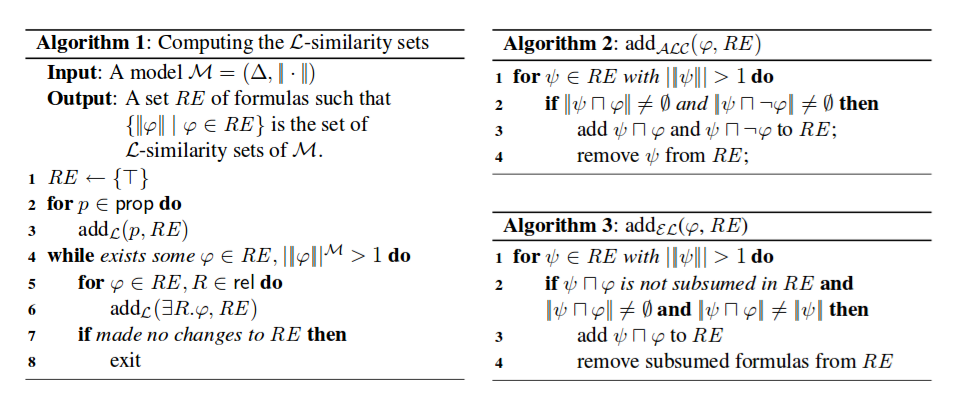
\includegraphics[width=\textwidth]{images/algoritmoOriginal.png}
%\end{center}
%\vspace*{-2em}
%\caption{Algoritmo para GER con l\'ogicas de descripci\'on}
%\label{algoritmoOriginal}
%\end{figure}

%\subsection{Ejemplo de ejecuci\'on}
%
%
%
%\textcolor{blue}{no se si poner aca un ejemplo, si poner el texto y las im\'agenes en otro apendice... o ponerlas mas chiquitas en varias columnas, asi queda feo}\\
%Vamos a ejecutar el algoritmo para la Figura~\ref{GRE3D7-stimulus-cap2},
%el algoritmo comienza con una lista fija de propiedades y relaciones, supongamos que
%esas listas son las siguientes:
%
%propiedades ordenadas (prop): \textsf{ball}, \textsf{cube}, \textsf{red}, \textsf{yellow}, \textsf{small}, \textsf{large}.\\
%relaciones ordenadas (rel): \textsf{leftof}, \textsf{rightof}, \textsf{ontopof}, \textsf{bellowof}.
%
%%\begin{figure}
%%\begin{center}	
%%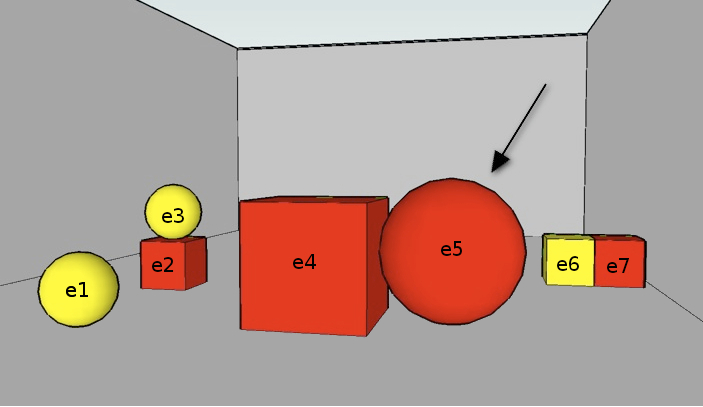
\includegraphics[width=.5\textwidth]{images/22.jpg}
%%\end{center}
%%\vspace*{-1.5em}
%%\caption{Escena 3D de figuras geom\'etricas}\label{figure22}
%%\end{figure}
%
%%\begin{figure}
%%\begin{minipage}[b]{0.6\linewidth}
%%\centering
%%\begin{tikzpicture}
%%  [
%%    n/.style={circle,fill,draw,inner sep=3pt,node distance=1.4cm},
%%    aArrow/.style={->, >=stealth, semithick, shorten <= 2pt, shorten >= 2pt},
%%  ]
%% \node[n,label=above:$e_1$,label=below:{
%%    \relsize{-1}$\begin{array}{c}
%%      \nLeft\\[-2pt]
%%      \nSmall\\[-2pt] 
%%      \nYellow \\[-2pt] 
%%      \nBall\end{array}$}] (a) {};
%
%% \node[n,label=above:$e_2$,label=below:{
%%    \relsize{-1}$\begin{array}{c}
%%      \nLeft\\[-2pt]
%%      \nSmall\\[-2pt] 
%%      \nRed\\[-2pt] 
%%      \nCube\end{array}$}, right of=a] (b) {};
%
%% \node[n,label=below:$e_3$,label=above:{
%%    \relsize{-1}$\begin{array}{c}
%%      \nTop\\[-2pt]
%%      \nLeft\\[-2pt]
%%      \nSmall\\[-2pt] 
%%      \nYellow\\[-2pt] 
%%      \nBall\end{array}$}, above of=b] (c) {};
%
%% \node[n,label=above:$e_4$,label=below:{
%%    \relsize{-1}$\begin{array}{c}
%%      \nBig\\[-2pt] 
%%      \nRed\\[-2pt] 
%%      \nCube\end{array}$}, right of=b] (d) {};
%
%% \node[n,label=above:$e_5$,label=below:{
%%    \relsize{-1}$\begin{array}{c}
%%      \nBig\\[-2pt] 
%%      \nRed\\[-2pt] 
%%      \nBall\end{array}$}, right of=d] (e) {};
%
%% \node[n,label=above:$e_6$,label=below:{
%%    \relsize{-1}$\begin{array}{c}
%%      \nSmall\\[-2pt] 
%%      \nYellow\\[-2pt] 
%%      \nCube\end{array}$}, right of=e] (f) {};
%
%% \node[n,label=above:$e_7$,label=below:{
%%    \relsize{-1}$\begin{array}{c}
%%      \nSmall\\[-2pt] 
%%      \nRed\\[-2pt] 
%%      \nCube\end{array}$}, right of=f] (g) {};
%
%% \draw [aArrow,bend right=90] (b) to node[auto,swap]{\relsize{-1}$\nBelow$} (c);
%% \draw [aArrow,bend right=90] (c) to node[auto,swap]{\relsize{-1}$\nOntop$} (b);
%
%% \draw [aArrow,bend right=30] (d) to node[auto,swap]{\relsize{-1}$\nLeftof$} (e);
%% \draw [aArrow,bend right=30] (e) to node[auto,swap]{\relsize{-1}$\nRightof$} (d);
%
%% \draw [aArrow,bend right=30] (f) to node[auto,swap]{\relsize{-1}$\nLeftof$} (g);
%% \draw [aArrow,bend right=30] (g) to node[auto,swap]{\relsize{-1}$\nRightof$} (f);
%
%% \draw[dotted] (-.4,-1.7) rectangle (7.5,3.3);
%
%% \end{tikzpicture}
%%\caption{La escena como modelo relacional}\label{GRE3D7-stimulus-graph}
%%\end{minipage}
%%\end{figure}
%
%
%El algoritmo siempre termina, y devuelve ER un conjunto de f\'ormulas que describe cada elemento en el dominio (si existe esa f\'ormula). \\
%
%En el comienzo ER=$\{\top\}$ y $\interp{\top}$ = $\{e_1, e_2, e_3, e_4, e_5, e_6, e_7\}$ como se puede ver en la Figura~\ref{fig-modelo}.\\
%
%ACA
%\begin{figure}[ht]
%\begin{minipage}[b]{0.45\linewidth}
%\centering
%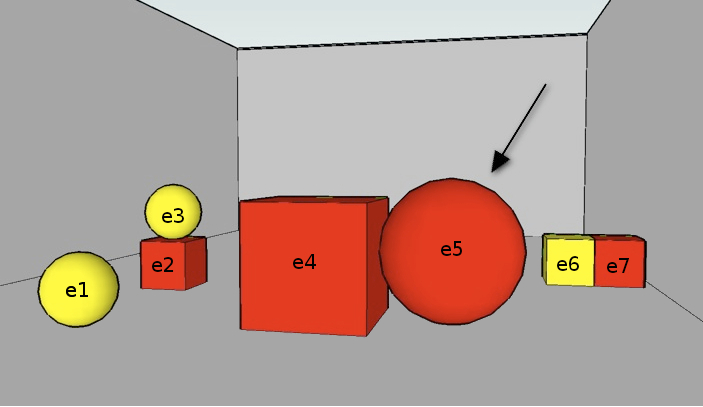
\includegraphics[width=\textwidth]{images/22.jpg}
%\vspace*{1cm}
%%\caption{Input scene}
%\label{GRE3D7-stimulus-22}
%\end{minipage}
%%\hspace*{-0.35cm}
%\begin{minipage}[b]{0.6\linewidth}
%\centering
%%\begin{figure}[ht]
%%\begin{center}
%\frame{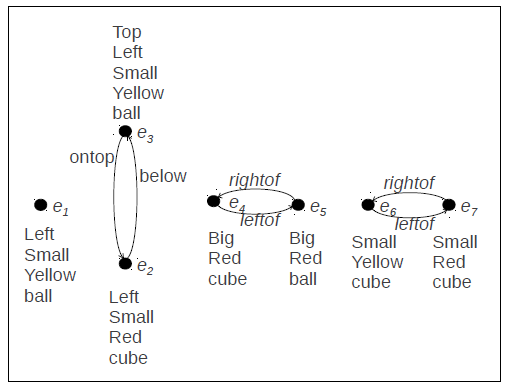
\includegraphics[width=8cm]{images/modelo.png}}\\[0pt]
%\caption{Modelo de la Figura \ref{GRE3D7-stimulus-22}}
%\label{fig-modelo}
%\end{minipage}
%\end{figure}
%El primer bucle del algoritmo es en las propiedades. Para cada propiedad hace add$_\el$ ($\varphi$, RE), las propiedades at\'omicas se muestran en la Figura~\ref{fig-modelo2}.
%
%\begin{figure}[ht]
%\begin{center}
%\frame{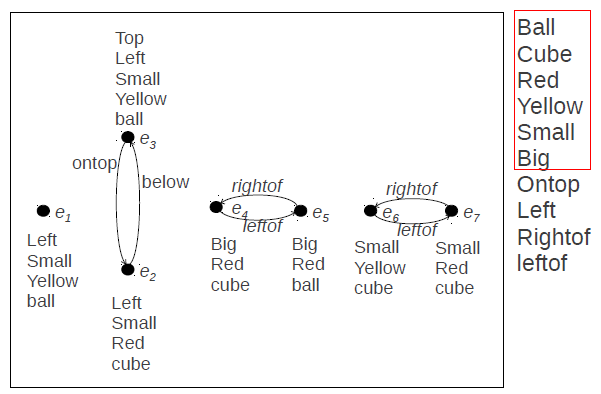
\includegraphics[width=8cm]{images/modelo2.png}}\\[0pt]
%\caption{Propiedades proposicionales en cuadro rojo, las del primer ciclo del algoritmo}
%\label{fig-modelo2}
%\end{center}
%\end{figure}
%
%La f\'ormula $\varphi$ se a\~nadir\'a a ER si su interpretaci\'on tiene al menos un elemento, a continuaci\'on, para cada f\'ormula
 %$\psi$ en ER la conjunci\'on
%$\varphi  \wedge \psi$ no necesita estar subsumida in ER, la $\interp{\varphi \cup \psi}$ no tiene que ser vac\'io, y su interpretaci\'on tiene que ser distinta de $\interp{\psi}$. Luego las f\'ormulas subsumidas se borran.
%
%La primer propiedad es \textsf{ball}, ER = \{$\top$, \textsf{ball}\}, se ven los elementos de ``ball'' en un recuadro en la Figura~\ref{fig-modelo3}.
%
%\begin{figure}[ht]
%\begin{center}
%\frame{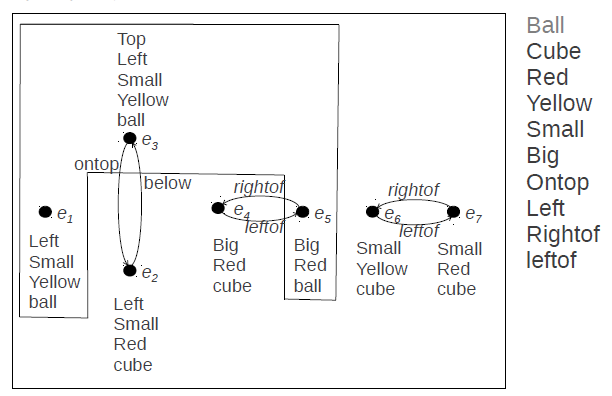
\includegraphics[width=8cm]{images/modelo3.png}}\\[0pt]
%\caption{El cuadro indica cuales son ``ball''}
%\label{fig-modelo3}
%\end{center}
%\end{figure}
%
%La siguiente propiedad es \textsf{cube}, ER = \{$\top$, \textsf{ball}, \textsf{cube}\}, pero ahora la $\interp{\textsf{ball}}$ = $\{e_1, e_3, e_5\}$, $\interp{\textsf{cube}}$ = $\{e_2, e_4, e_6, e_7\}$, quedando las particiones como se muestra en la Figura~\ref{fig-modelo4}
%\begin{figure}[ht]
%\begin{center}
%\frame{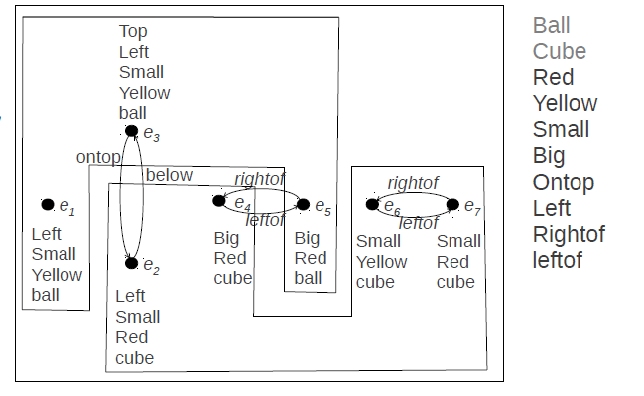
\includegraphics[width=8cm]{images/modelo4.png}}\\[0pt]
%\caption{Cuadros indicando ``ball'' y ``cube''}
%\label{fig-modelo4}
%\end{center}
%\end{figure}
%Ahora podemos borrar $\top$, porque es subsumida (esta cubierta por) las otras dos f\'ormulas. La siguiente propiedad es  \textsf{red}, $\interp{\textsf{red}}$ es: $\{e_2, e_4, e_5, e_7\}$, haciendo la intersecci\'on con la $\interp{.}$ de cada f\'ormula en ER obtenemos, $\{e_5\}$ y $\{e_2, e_4, e_7\}$, ER = $\{\textsf{ball}, \textsf{cube}, \textsf{ball} \wedge \textsf{red}, \textsf{cube} \wedge \textsf{red}\}$, las particiones actuales se pueden ver en la Figura~\ref{fig-modelo9}.
%\begin{figure}[ht]
%\begin{center}
%\frame{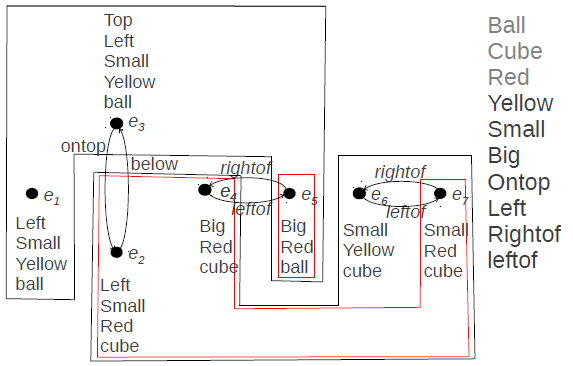
\includegraphics[width=8cm]{images/modelo9.png}}\\[0pt]
%\caption{Cuadros indicando ``ball'', ``cube'' y ``red''}
%\label{fig-modelo9}
%\end{center}
%\end{figure}
%
%Siguiendo con \textsf{yellow}, tenemos, $\interp{\textsf{yellow}}$ = $\{e_1, e_3, e_6\}$ y obtenemos ER = $\{\textsf{ball} \wedge \textsf{yellow}, \textsf{cube} \wedge \textsf{yellow}, \textsf{ball} \wedge \textsf{red}, \textsf{cube} \wedge \textsf{red}\}$. 
%Note que aqu\'i ya borramos la f\'ormula \textsf{ball} porque estaba subsumida, y la f\'ormula \textsf{cube} tambi\'en. Se muestran particiones en Figura~\ref{fig-modelo10}.
%
%\begin{figure}[ht]
%\begin{center}
%\frame{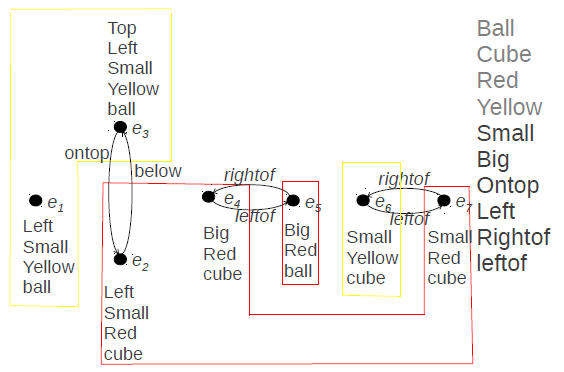
\includegraphics[width=8cm]{images/modelo10.png}}\\[0pt]
%\caption{Cuadros indicando ``ball'', ``cube'', ``red'' y ``yellow''}
%\label{fig-modelo10}
%\end{center}
%\end{figure}
%
%Haciendo lo mismo con \textsf{small} tenemos ER = $\{\textsf{ball} \wedge \textsf{yellow} \wedge \textsf{small}, \textsf{cube} \wedge \textsf{yellow} \wedge \textsf{small}, \textsf{ball} \wedge \textsf{red}, \textsf{cube} \wedge \textsf{red}, \textsf{cube} \wedge \textsf{red} \wedge \textsf{small}\}$, como se puede ver en Figura~\ref{fig-modelo11}.
%\begin{figure}[ht]
%\begin{center}
%\frame{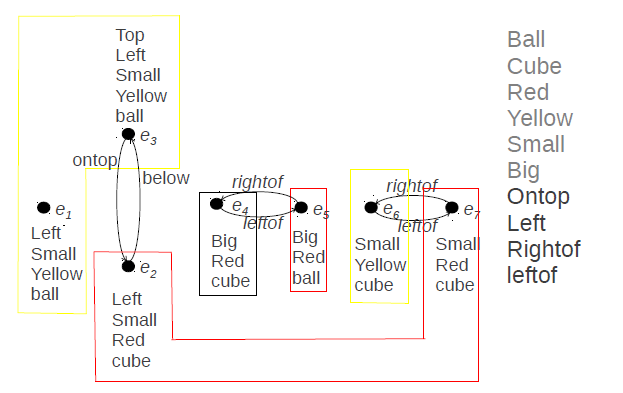
\includegraphics[width=8cm]{images/modelo11.png}}\\[0pt]
%\caption{Cuadros indicando ``ball'', ``cube'', ``red'', ``yellow'', ``small'' y ``large''}
%\label{fig-modelo11}
%\end{center}
%\end{figure}
%
%La siguiente propiedad es \textsf{large} as\'i, tenemos ER = $\{\textsf{ball} \wedge \textsf{yellow} \wedge \textsf{small}, \textsf{cube} \wedge \textsf{yellow} \wedge \textsf{small}, \textsf{ball} \wedge \textsf{red}, \textsf{cube} \wedge \textsf{red} \wedge \textsf{large}, \textsf{cube} \wedge \textsf{red} \wedge \textsf{small}\}$. Aqu\'i no podemos agregar \textsf{large} a la f\'ormula $\textsf{red} \wedge \textsf{cube}$ porque su interpretaci\'on tiene un solo elemento, y la condici\'on dice que es necesario tener m\'as de uno.
%
%Hasta ahora ER = $\{\textsf{ball} \wedge \textsf{yellow} \wedge \textsf{small}, \textsf{cube} \wedge \textsf{yellow} \wedge \textsf{small}, \textsf{ball} \wedge \textsf{red}, \textsf{cube} \wedge \textsf{red} \wedge \textsf{large}, \textsf{cube} \wedge \textsf{red} \wedge \textsf{small}\}$ 
%y tenemos las siguientes extensiones: $\{e_1, e_3\}, \{e_6\}, \{e_5\}, \{e_4\}, \{e_2, e_7\}$ respectivamente. 
%Hay dos f\'ormulas que a\'un pueden ser refinadas, $\textsf{ball} \wedge \textsf{yellow} \wedge \textsf{small}$ y $\textsf{cube} \wedge \textsf{red} \wedge \textsf{small}$ 
%debido a que tienen m\'as de un elemento cada una, por lo que entran en el ciclo, while del algoritmo 1, en la l\'inea 4. Ahora es el turno de las relaciones, la primera de ellas es \textsf{leftof}, para cada f\'ormula $\varphi$ en ER trataremos de hacer add$_\el$ ($\exists \textsf{leftof}.\varphi$, RE). Notar que $\psi$ solo puede ser $\textsf{ball} \wedge \textsf{yellow} \wedge \textsf{small}$ o $\textsf{cube} \wedge \textsf{red} \wedge \textsf{small}$ porque esos son los que su interpretaci\'on tiene m\'as de un elemento. 
%\begin{figure}[ht]
%\begin{center}
%\frame{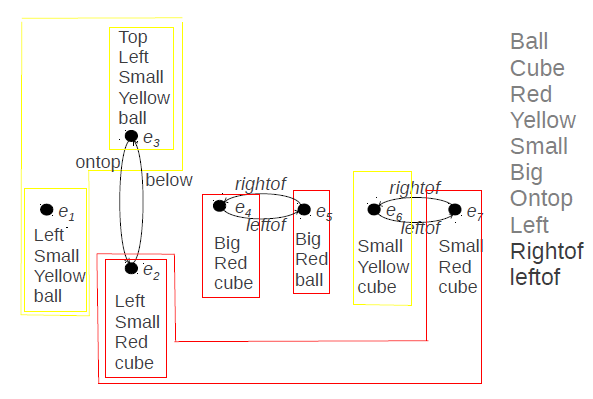
\includegraphics[width=8cm]{images/modelo15.png}}\\[0pt]
%\caption{Cuadros indicando ``ball'', ``cube'', ``red'', ``yellow''...}
%\label{fig-modelo15}
%\end{center}
%\end{figure}
%
%
%No hay
%%because those are the ones that its interpretation have more than one element. There is not 
%$\varphi$ y $\psi$ que puedan ser aplicadas. Continuando con \textsf{rightof} agregamos $\textsf{cube} \wedge \textsf{yellow} \wedge \textsf{small} \wedge \exists \textsf{rightof}. \textsf{cube} \wedge \textsf{red} \wedge \textsf{small}$, y asi con \textsf{topof} agregamos $\textsf{small} \wedge \textsf{red} \wedge \textsf{cube} \wedge \exists \textsf{ontop}. \textsf{small} \wedge \textsf{yellow} \wedge \textsf{ball}$ y el algoritmo termina con ER = $\{\textsf{ball} \wedge \textsf{yellow} \wedge \textsf{small}, \textsf{cube} \wedge \textsf{yellow} \wedge \textsf{small}, \textsf{ball} \wedge \textsf{red}, \textsf{cube} \wedge \textsf{red} \wedge \textsf{large}, \textsf{cube} \wedge \textsf{red} \wedge \textsf{small}, \textsf{cube} \wedge \textsf{yellow} \wedge \textsf{small} \wedge \exists \textsf{rightof}. \textsf{cube} \wedge \textsf{red} \wedge \textsf{small}, \textsf{small} \wedge \textsf{red} \wedge \textsf{cube} \wedge \exists \textsf{ontop}. \textsf{small} \wedge \textsf{yellow} \wedge \textsf{ball}\}$, 
%aqu\'i todos los elementos est\'an en una clase singleton y no se puede hacer ning\'un refinamiento m\'as. 
%%can be applied to $cube \wedge red \wedge small$ but there is no formula which interpretation has more than one element to be apply with this one. The same happen for the other relations, so the algorithm ends.
%%its interpretation is $\{e_7\}$ with $\psi$ is $cube \wedge yellow \wedge small$, the others combinations can't be apply because they don't do true the preconditions. The following relation is rightof, 
%
%%leftof, rightof, ontopof, bellowof
%
%%At this point we already have the target in a singleton set. So the formula for it is ``red and ball'', and also for s6 which formula is ``yellow cube''.\\
%%As we show this algorithm depends of the order of properties and relations.\\
%\begin{figure}[ht]
%\begin{center}
%\frame{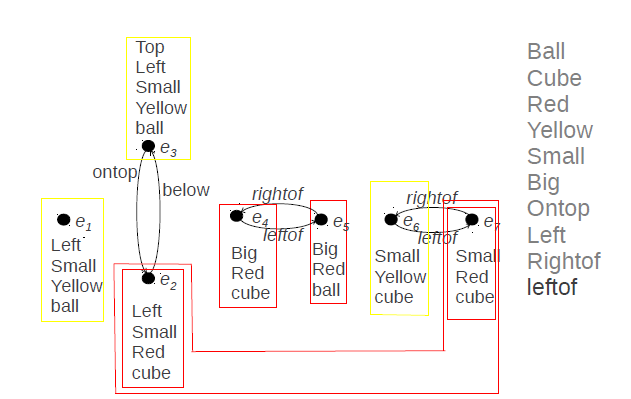
\includegraphics[width=8cm]{images/modelo16.png}}\\[0pt]
%\caption{Cuadros indicando ``ball'', ``cube'', ``red'', ``yellow''...}
%\label{fig-modelo16}
%\end{center}
%\end{figure}
%
%\begin{figure}[ht]
%\begin{center}
%\frame{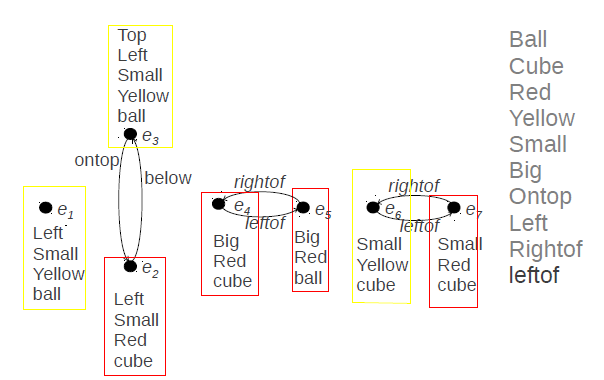
\includegraphics[width=8cm]{images/modelo17.png}}\\[0pt]
%\caption{Cuadros indicando ``ball'', ``cube'', ``red'', ``yellow''...}
%\label{fig-modelo17}
%\end{center}
%\end{figure}
%
%Las expresiones referenciales encontradas son:\\
%
%$\textsf{ball} \wedge \textsf{yellow} \wedge \textsf{small}$ representa $e_1$ \\
%$\textsf{cube} \wedge \textsf{yellow} \wedge \textsf{small}$ representa $e_6$ \\
%$\textsf{ball} \wedge \textsf{red}$ representa $e_5$ \\
%$\textsf{cube} \wedge \textsf{red} \wedge \textsf{large}$ representa $e_4$ \\
%$\textsf{cube} \wedge \textsf{red} \wedge \textsf{small}$ representa $\{e_2,e_7\}$  \\
%$\textsf{cube} \wedge \textsf{yellow} \wedge \textsf{small} \wedge \exists \textsf{rightof}. \textsf{cube} \wedge \textsf{red} \wedge \textsf{small}$ representa $e_6$ \\
%$\textsf{small} \wedge \textsf{red} \wedge \textsf{cube} \wedge \exists \textsf{ontop}. \textsf{small} \wedge \textsf{yellow} \wedge \textsf{ball}$ representa $e_2$ \\
%



\section{Aproximaciones emp\'iricas a la soluci\'on de GER}

\subsection{Corpus existente}
\label{sec:corpus2}
\label{sec:corpusTUNA}

%was the first prominent REG corpus to be made publicly available for research purposes. The corpus was developed in a series of general-purpose controlled experiments, containing 2280 descriptions produced by 60 speakers in two domains (1200 descriptions of furniture items and 1080 descriptions of people's photographs). TUNA does not contain relational descriptions, and it is possibly the only resource of this kind to include situations of reference to sets. The TUNA corpus has been extensively used in a series of shared tasks

TUNA \cite{tuna-corpus} fue el primer corpus prominente para GER disponible p\'ublicamente con fines de investigaci\'on. El corpus fue desarrollado en una serie de experimentos controlados de prop\'osito general, contiene 2.280 descripciones producidas por 60 personas en dos dominios (1.200 expresiones referenciales de im\'agenes de muebles y 1080 expresiones referenciales de fotograf\'ias de personas situadas en una grilla). Se muestran ejemplos de im\'agenes en Figuras \ref{fig-TUNA-furniture} y \ref{fig-TUNA-people}. El corpus TUNA no contiene descripciones relacionales, y es posiblemente el \'unico recurso de este tipo que incluye situaciones de referencia a conjuntos. Este corpus se ha utilizado ampliamente en una serie de desaf\'ios \cite{reg2009}. \\

\begin{figure}
\begin{minipage}[t]{0.5\linewidth}
\centering
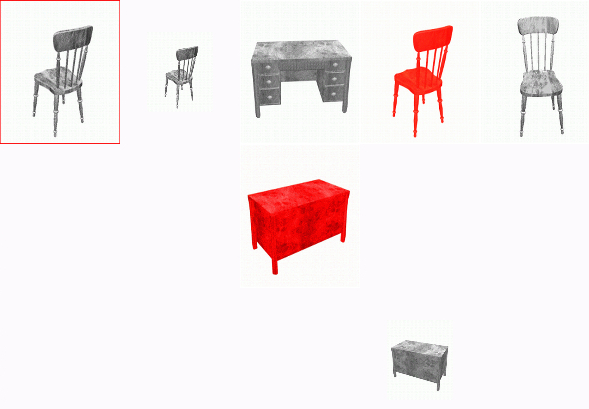
\includegraphics[width=\textwidth]{images/largeGreyChair.jpg}\\[0pt]
\caption{Imagen del TUNA corpus (muebles)}
\label{fig-TUNA-furniture}
\vspace*{.1cm}
\end{minipage}
\hspace*{0cm}
\begin{minipage}[t]{0.5\linewidth}
\centering
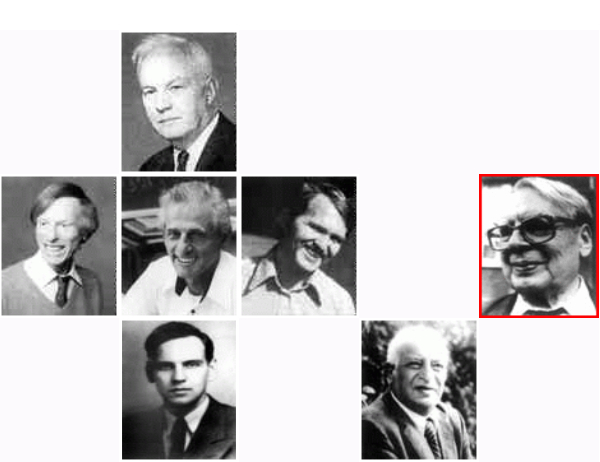
\includegraphics[width=\textwidth]{images/tuna-people.jpg}\\[0pt]
\caption{Imagen del TUNA corpus (personas)}
\label{fig-TUNA-people}
\end{minipage}
\end{figure}


\label{sec:corpusGRE}
%were developed in a series of web-based experiments primarily focussed on the study of relational descriptions. GRE3D3 contains 630 descriptions produced by 63 speakers, and GRE3D7 contains 4480 descriptions produced by 287 speakers, making it the largest of its kind to date. The GRE3D domain consists of simple visual scenes containing only two kinds of objects (boxes and spheres) with limited variation in colour and size. In each scene, there is only one possible spatial relation between target and the nearest landmark. Both corpora contain atomic and relational descriptions.
GRE3D3 y su extensi\'on GRE3D7 \cite{gre3d3,gre3d7} se desarrollaron en una serie de experimentos basados en la web, se centraron principalmente en el estudio de las descripciones relacionales. GRE3D3 contiene 630 descripciones producidas por 63 personas y GRE3D7 contiene 4.480 descripciones producidas por 287 personas, y es el corpus m\'as grande de este tipo hasta la fecha. El dominio del GRE3D3 consta de escenas visuales simples que contienen s\'olo dos tipos de objetos (cubos y esferas) con variaci\'on limitada en color y tama\~no. En cada escena, s\'olo hay una posible relaci\'on espacial entre el target y el landmark m\'as cercano. Ambos corpus contienen descripciones at\'omicas y relacionales. Ejemplo de im\'agenes del GRE3D3 y GRE3D7 se muestran en las Figuras \ref{fig-GRE3D3} y \ref{fig-GRE3D7}.\\
%\begin{minipage}[b]{0.45\linewidth}

\begin{figure}
\begin{minipage}[b]{0.5\linewidth}
\centering
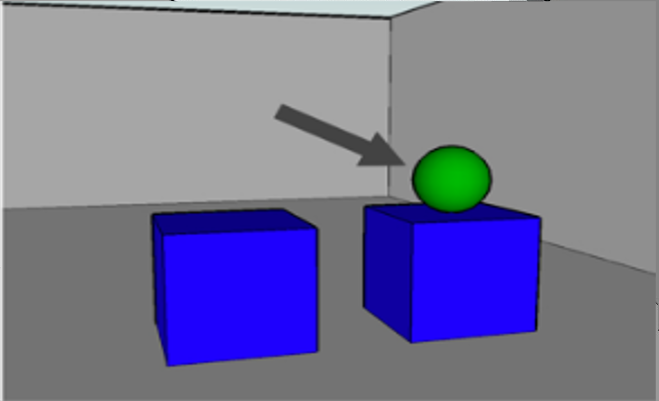
\includegraphics[width=\textwidth]{images/GRE3D3.png}\\[0pt]
\caption{Imagen del GRE3D3}
\label{fig-GRE3D3}
\vspace*{-0.7cm}
\end{minipage}
\hspace*{0cm}
\begin{minipage}[b]{0.5\linewidth}
\centering
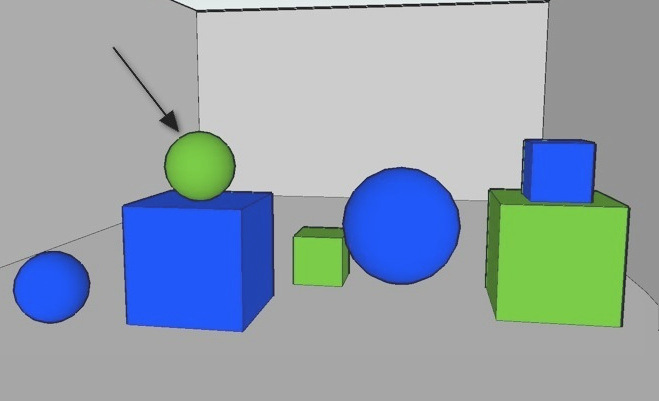
\includegraphics[width=\textwidth]{images/3.jpg}\\[0pt]
\caption{Imagen del GRE3D7}
\label{fig-GRE3D7}
\end{minipage}
\end{figure}

%\vspace*{3cm}

\label{sec:corpusSTARS}
%and its extension Stars2 were collected for the study of referential overspecification (particularly in the case of relational descriptions). Stars was developed in a pilot web-based experiment, containing 704 descriptions produced by 64 speakers.  The more comprehensive Stars2 data set was produced in dialogue situations involving subject pairs, and it contains 884 descriptions produced by 56 speakers. Both domains make use of simple visual scenes containing up to four object types (e.g., stars, boxes, cones and spheres) with limited variation in colour and size. Differently from other REG corpora, however, Stars/2 includes a considerable number of complex situations of reference involving up to three objects, as in `the box near the sphere, next to the cone'.http://ppgsi.each.usp.br/arquivos/RelTec/PPgSI-002_2014.pdf y http://ppgsi.each.usp.br/arquivos/RelTec/PPgSI-001_2015.pdf
Stars \cite{stars-mutual-disamb} y su extensi\'on Stars2 se colectaron para el estudio de la sobre-especificaci\'on (particularmente en el caso de las descripciones relacionales). Stars se desarroll\'o en un experimento piloto basado en la web, contiene 704 descripciones producidas por 64 personas. El conjunto de datos Stars2 es m\'as completo y se obtuvo de situaciones de di\'alogo que implicaban a dos personas, contiene 884 descripciones producidas por 56 participantes. Ambos dominios hacen uso de escenas visuales simples que contienen tres tipos de objetos (por ejemplo para Stars, estrellas, cuadrados y c\'irculos y para Stars2 cubos, conos y esferas) con variaci\'on limitada en color y tama\~no. A diferencia de otros corpus para GER, Stars/2 incluyen un n\'umero considerable de situaciones complejas de referencia en que participan hasta tres objetos, como en ``el cubo cerca de la esfera, al lado del cono''. Ejemplos de imagenes se muestran en las Figuras \ref{fig-STARS} y \ref{fig-STARS2}.\\


\begin{figure}
\begin{minipage}[b]{0.5\linewidth}
\centering
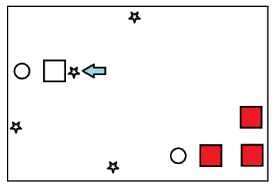
\includegraphics[width=\textwidth]{images/STARS.png}\\[0pt]
\caption{Imagen de Stars corpus}
\label{fig-STARS}
%\vspace*{1cm}
\end{minipage}
\hspace*{0cm}
\begin{minipage}[b]{0.5\linewidth}
\centering
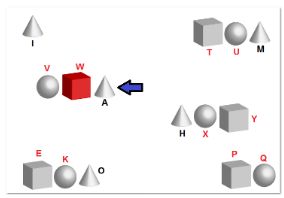
\includegraphics[width=\textwidth]{images/STARS2.png}\\[0pt]
\caption{Imagen de Stars2 corpus}
\label{fig-STARS2}
\end{minipage}
\end{figure}

%ejemplo minipage
%\begin{figure}
%\begin{minipage}[b]{0.5\linewidth}
%\centering
%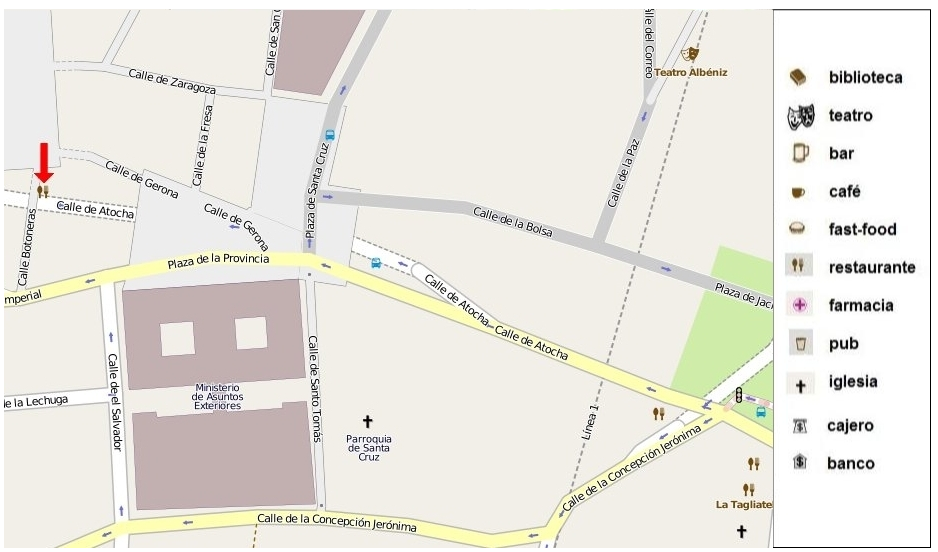
\includegraphics[width=\textwidth]{figures/rest-singular2x.png}\\[0pt]
%\caption{Target singular con zoom 2X}
%\label{rest-singular2x}
%\end{minipage}
%\vspace*{.1cm}
%\begin{minipage}[b]{0.5\linewidth}
%\centering
%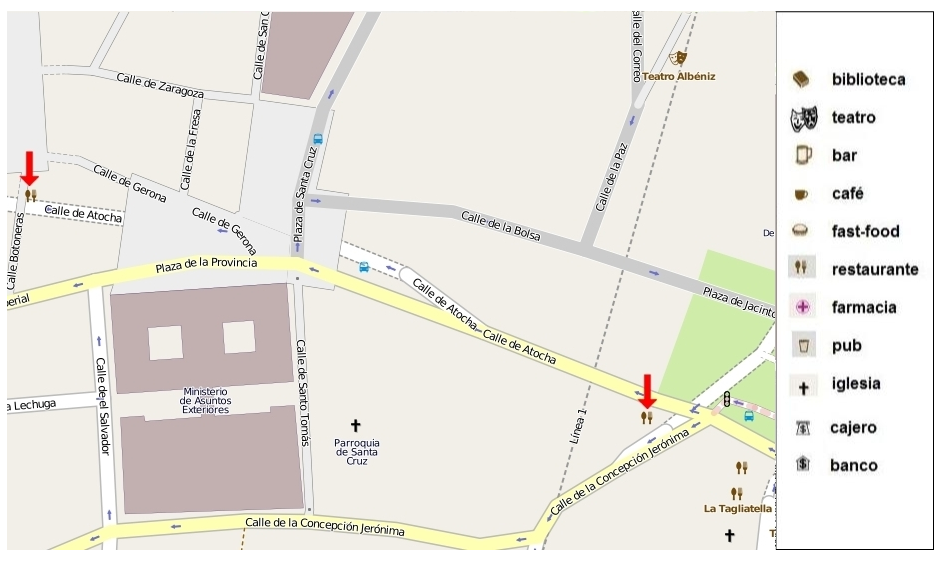
\includegraphics[width=\textwidth]{figures/rest-plural2x.png}\\[0pt]
%\caption{Target plural con zoom 2X}
%\label{rest-plural2x}
%\end{minipage}
%\end{figure}




%Despite their usefulness and general contribution to the research in REG, the above domains are still at a certain distance from the kinds of visual scene that might be required for a practical, real-world application. The need for additional complexity and/or realism, and our own interest in the surface realisation task for the Spanish and Portuguese languages, has led us to build a new computational resource of this kind. This work is described in the next sections. Further discussion on the differences between the Zoom corpus and existing resources is presented in Sec. \ref{sec-annotation}. 



\subsection{Trabajos emp\'iricos en el \'area}

%http://link.springer.com/chapter/10.1007/978-3-642-15573-4_9
%http://www.jetteviethen.net/papers/DaleViethen2010chapter.pdf

La investigaci\'on presentada en \cite{viethen-phd} se basa en dos premisas fundamentales: que la investigaci\'on
en la generaci\'on autom\'atica de expresiones referenciales debe esforzarse por lograr
sistemas que den salidas tan similar a la humana como sea posible; y que, para ello, debemos
esforzarnos para modelar el comportamiento humano como se puede observar en corpora.

La adopci\'on de estas premisas sirve para dos fines: en primer lugar, mejora la adecuaci\'on
de la salida de algoritmos de GER para el objeto target imitando la capacidad humana
de producir referencias adecuadas; y en segundo lugar, el estudio de corpus de datos producidos por humanos
 y algoritmos en desarrollo que pueden replicar estos datos podr\'ian
acercarnos a la comprensi\'on de que es lo que hacen los humanos cuando dan una ER.\\

Se\~nala que el cl\'asico algoritmo de GER y la mayor parte de sus descendientes no se basaron ni evaluaron contra datos producidos por humanos. Ellos se basaron en una visi\'on bastante minimalista de lo que se necesita
para que una expresi\'on referencial sea \'optima, concentr\'andose en la eficiencia computacional 
 y descripciones breves como sus principales preocupaciones.\\

 Existe un peque\~no n\'umero de enfoques que 
 se basaron en observaciones del comportamiento de referencia general humana
que obtuvieron a partir de experimentos psicoling\"u\'isticos, pero de nuevo no fueron evaluados
contra datos humanos.\\

Los algoritmos que se presentaron a los desaf\'ios de evaluaci\'on \cite{gatt-balz-kow:2008:ENLG} y \cite{reg2009}
fueron probados en el TUNA-Corpus, y algunos de ellos
tambi\'en tuvieron en cuenta los patrones que se encontraban en el conjunto del desarrollo. Pero hay una serie de preocupaciones en torno a la pregunta de si el TUNA-Corpus, y la forma de salida de los sistemas que se compar\'o 
en los desaf\'ios eran ideales para una evaluaci\'on de la adecuaci\'on descriptiva de GER.\\
%saque esto porque no se entiende
%A partir de los desaf\'ios que se describen en m\'as detalle y para evaluarlos en una serie de datos m\'as grande
%que contiene m\'as de una expresi\'on referencial para cada elemento est\'imulo.
Aborda tres \'areas principales en las que los corpus se puede utilizar para
promover el objetivo de la semejanza humana en la investigaci\'on sobre generaci\'on de expresiones referenciales:
evaluaci\'on, la recolecci\'on de corpus y an\'alisis y modelizaci\'on estad\'istica de
datos de corpus.\\
Comenz\'o con el an\'alisis del estado del arte de la investigaci\'on en
la generaci\'on de descripciones distintivas, trabaj\'o con relaciones espaciales y en el trabajo us\'o datos de corpus. Examin\'o una serie de opciones metodol\'ogicas que tienen que hacerse cuando se trabaja con los corpus de GER. Aqu\'i, explor\'o diferentes opciones para los desaf\'ios de recopilaci\'on de corpus, que se centran en torno al equilibrio que se necesita
entre el control de los par\'ametros experimentales tanto como sea necesario
y mantener la configuraci\'on de lo m\'as natural posible. Discuti\'o una serie de conceptos
que son de importancia para el an\'alisis de corpora de GER, tales como la naturalidad de diferentes
propiedades de los objetos, y las nociones de minimalidad y cuestiones de sobre-especificaci\'on de expresiones referenciales. Por \'ultimo, analiz\'o diferentes maneras en que la salida de un sistema se puede
comparar con los datos de corpora, bajo la premisa de que el objetivo de la comparaci\'on es
para evaluar si el sistema podr\'ia tener un modelo adecuado del comportamiento humano para la generaci\'on de expresiones referenciales.
Realiz\'o una investigaci\'on en las tres \'areas donde se puede emplear corpora en GER: Evaluaci\'on de semejanza humana, recopilaci\'on y an\'alisis de corpus, y modelado de datos de corpus. Realiz\'o un experimento de evaluaci\'on con tres de los algoritmos cl\'asicos, (1989) Algoritmo Greedy de Dale (Greedy), Dale y Haddock (1991b), Algoritmo Relacional (ra) Y Dale y Reiter (1995) Algoritmo Incremental (IA), Se pusieron a prueba en cuanto a su capacidad de
replicar las expresiones referenciales se encuentran en un grupo relativamente peque\~no de corpus de expresiones referenciales
en un dominio visual de im\'agenes puestas en una grilla.
%de rejilla de cajones de armarios ling. 
En el an\'alisis de este experimento tuvo dos resultados principales: (1) que identic\'o en particular tres 
fen\'omenos que todav\'ia plantean importantes retos para los algoritmos GER con el objetivo de replicar
el comportamiento humano, y (2) que proporciona una plataforma para la discusi\'on de una serie de
dificultades que se presentan para la evaluaci\'on basada en corpus de GER. Esto result\'o en una serie
de criterios para el dise\~no de los dos corpus que el trabajo en el resto de la tesis.
Los tres fen\'omenos en las expresiones referenciales producidas por humanos que los
algoritmos probados no fueron capaces de replicar satisfactoriamente sobre-especificaci\'on,
relaciones espaciales, y comportamiento de voluntarios espec\'ificos. Ambos
Greddy y la IA fueron capaces de generar algo de la redundancia que se encontr\'o en el corpus.
 Ni Greedy ni el IA estaban dise\~nados para ser capaz de generar expresiones referenciales que contengan relaciones entre entidades, pero el ra fue dise\~nado para incluirlas. Sorprendentemente, el
ra no s\'olo fallo en generar cualquiera de las descripciones contenidas en el corpus de evaluaci\'on; sino tambi\'en que las descripciones que se gener\'o parec\'ian m\'as como enigmas cuyo objetivo era confundir a un oyente, m\'as que ayudar en
los intentos de se\~nalar el objetivo referente. 

Una valoraci\'on te\'orica de otras aproximaciones dise\~nados para manejar las relaciones estableci\'o que ninguno de ellos incluir\'ia una relaci\'on, si no es absolutamente necesaria para distinguir el target.
La tercera observaci\'on que el experimento dejo a la vista fue que la gente no siempre hace lo mismo en la misma situaci\'on. De hecho, incluso la misma persona podr\'ia describir el mismo target de diferente manera en distintas
circunstancias. 

 None of the algorithms tested were intended to take such inter- and
intra-speaker variation into account, and only very recently have implementations
of the
ia
begun to model speaker-preferences to some degree.

No se pretend\'ia que ninguno de los algoritmos de la prueba tomara en cuenta las variaciones entre-hablantes, ni del mismo hablante. Hay implementaciones del IA que han comenzado a agregar modelo de preferencias de hablante en alg\'un grado.

Los temas generales con evaluaci\'on basada en corpus que esta experiencia de evaluaci\'on dej\'o
al descubierto fueron (1) la interdependencia estrecha entre algoritmos y la
representaci\'on subyacente de conocimiento que utilizan, (2) el no-determinismo de la generaci\'on del lenguaje natural, (3) la cuesti\'on de c\'omo comparar la salida algoritmos con gold-standar, y (4) el dominio espec\'ifico de los algoritmos de GER.\\
La discusi\'on de estos temas ha dado lugar a la siguiente lista de Evaluaci\'on en GER basado en corpus:

1. Si el corpora est\'a destinado para ser reutilizado para la evaluaci\'on comparativa de diferentes
algoritmos, una representaci\'on subyacente del dominio debe ser proporcionada para ser usada por todos los algoritmos.

2. Si queremos confiar en los resultados, el corpus debe contener tantos casos como sea posible de tantos direntes hablantes como sea posible para cada escenario referencial. 
Esto es cierto si un algoritmo es evaluado en t\'erminos de ser capaz de generar una expresi\'on referencial que suene natural, o si est\'a probado por su probabilidad de pertenecer a un modelo espec\'ifico de conducta humana de referencia, mediante la comprobaci\'on de si se puede generar todas las descripciones en un corpus.

3. Si la probabilidad de un algoritmo de ser un modelo de la conducta humana de referencia
se eval\'ua, deben utilizarse m\'etricas basadas en recuento (RECALL) y precisi\'on (PRESITION). En este
caso, el conjunto completo de las descripciones que el algoritmo proporciona para cada
escenario de referencia en virtud de cualquier ajuste de par\'ametro debe ser comparado con el
conjunto de las descripciones contenidas en el corpus para el mismo escenario referencial.
Si la capacidad m\'as orientada a la aplicaci\'on para generar una referencia es similar a la humana
se ha de evaluar, s\'olo una descripci\'on por escenario.
Esto debe hacerse utilizando m\'etricas basadas en la precisi\'on para probar c\'omo muchos de las
descripciones dadas por los algoritmos est\'an contenidas en el corpus.
4. Algoritmos que son juzgados en un dominio espec\'ifico c, no se debe asumir como
f\'acilmente adaptable a otros dominios. Idealmente, los corpus que abarcan muchos diferentes
deben estar disponibles para las pruebas de los algoritmos que generalizan en distintos tipos de dominios.
Realiz\'o 2 corpus el GRE3D3 y el GRE3D7 descriptos en \ref{sec:corpus2}

Trabaj\'o con \'arboles de decisi\'on ...
\textcolor{blue}{Aca agregar otras personas que usaron corpus para generacion de ER, Ivandre... }

%http://www.lrec-conf.org/proceedings/lrec2012/pdf/152_Paper.pdf
En el trabajo \ref{ivandre-work-corpus} presentan 2 alternativas para aprender la seleccio\'on de atributos de una expresi\'on referencial a partir de corpus. Toma los caracter\'isticas de aprendizaje como el conjunto de valores enteros que representan el poder discriminativo de cada atributo (es decir, el n\'umero de distractores que cada atributo elimina por cada atributo que tiene el target, ejemplos son color, tama\~no, etc.) 
 %For instance, in a context set as
%seen in previous Example 1, assuming that we would like to
%refer to E4, the corresponding discriminatory power values
%would be defined as d type =1, d size =1 and d colour =3.
%In the first learning method, we will attempt to learn possible
%Pj orderings (defined as nominal values) that, if applied
%to  the  Incremental  algorithm,  would  produce  the  desired
%output L for each given input C. In the second method, we
%will  use  the  input  C  to  (binary)  decide  whether  to  select
%each attribute individually.  We will call these our
%Global and Individual AS  classifiers,  which  are  discussed  sepa-
%rately below

\subsection{M\'etricas de evaluaci\'on/comparaci\'on con corpus}

Jordan y Walker usaron 25 veces la validaci\'on cruzada en 393 expresiones referenciales
de 13 de la Coco di\'alogos para probar diferentes combinaciones de caracter\'isticas. Ellos
medido la precisi\'on absoluta, siendo \'esta la proporci\'on de expresiones referenciales
generadas que son id\'enticas a las descripciones de referencia humanos producidos a partir de
el corpus. En el aislamiento, la intencional uencias factores desempe\~naron mejor (42,4\%
exactitud) que los otros dos conjuntos de caracter\'isticas (conjuntos de contraste: 30,4\% y conceptual
pactos: 28,9\%) y la combinaci\'on de los tres tipos de caracter\'isticas hicieron signicativa no inexactitud aumento (43,2\%). Sin embargo, lo que tuvo el mayor impacto fue cuarto,
independiente de la teor\'ia, el tipo de caracter\'isticas que registran informaci\'on al juicio espec\'ifico c, tales
como el juicio
Identificaci\'on
, El participante-diada, el hablante actual y el atributo exacta
valores de la referente de destino. En el aislamiento, esta colecci\'on de caracter\'isticas logra el 54,5\%
exactitud, y combin\'andolos con todos los otros tres tipos de caracter\'isticas s\'olo aumentaron
esta actuaci\'on al 59,9\%. Estos resultados apoyan leve a Jordan intencional
en
influencias modelo sobre los otros dos modelos, pero m\'as fuertemente sugieren que ninguno
de los modelos de capturar la variaci\'on en los datos muy bien
incursi\'on en el uso de la m\'aquina de aprendizaje para
reg
fue hecha por Stoia et al.
(2006). Ellos apuntan a la construcci\'on de un sistema de di\'alogo para un agente situado dando
instrucciones en un mundo virtual en 3D. Sin embargo, este enfoque no se centr\'o por lo
tanto en la selecci\'on de contenidos como en determinar la mejor forma de referencia a utilizar.
Utilizaron un aprendiz m\'aquina para entrenar a los \'arboles de decisi\'on que decidieron que determinador
utilizar, qu\'e tipo de cabeza para incluir en el sintagma nominal (por ejemplo, un pronombre o una
nombre com\'un) y si desea o no utilizar una frase modi sustantivo. La sem\'antica
contenido del modificador no estaba en cuesti\'on. Las funciones disponibles para la decisi\'on
alumnos de los \'arboles eran una mezcla de la historia del di\'alogo, contexto visual y tipo sem\'antico
informaci\'on sobre el referente objetivo. Entrenaron \'arboles de decisi\'on separados para de-
terminer, sustantivo principal y la elecci\'on modificador y les aplicaron secuencialmente, con cada \'arbol que tenga acceso a la salida del \'arbol anterior. Para el entrenamiento y autom\'atico
%evaluaci\'on que utilizan un conjunto de 1242 expresiones referenciales de una colecci\'on de di\'alogo
%Logues entre dos compan\~eros de conversaci\'on que llevaban a cabo la instrucci\'on
%tarea en el mismo mundo virtual como el sistema se emplea en adelante. Esta
%evaluaci\'on autom\'atica encontr\'o que los \'arboles de decisi\'on fueron capaces de igualar la humana datos en el 31\% de todos los casos. Como no estaban interesados ​​tanto en la semejanza humana
%de su sistema, pero sobre todo en su cacia e, tambi\'en realizaron un intr\'inseca
%Evaluaci\'on humana en la que se pidi\'o a los participantes para comparar la salida del sistema
%a las expresiones que se refieren humanos producidos en una l\'inea de base y al azar. El humano
%evaluadores juzgados 62,6\% de las expresiones que se refieren generados por el sistema para


Un n\'umero de los sistemas presentados a la reg desaf\'ios de evaluaci\'on basados
en el at\'un
Corpus se basaron en los an\'alisis emp\'iricos del conjunto de entrenamiento. La mayor\'ia
de estos sistemas se basaban en la
ia y se utiliza un simple recuento de frecuencia de la
propiedades en el conjunto de entrenamiento para informar el orden en que Propie- del referente de destino
propie- deben ser juzgados (Kelleher, 2007; Spanger et al, 2007;. Fabbrizio et al., 2008;
Kelleher y Namee, 2008; de Lucena y Paraboni, 2008; Gerv como et al, 2008?.;
de Lucena y Paraboni, 2009). Un equipo, que yo era parte de, que se utiliza en frecuencia
funciones basadas en costos en el algoritmo gr\'afico-Based (Theune et al, 2007; Krahmer.
et al., 2008; Brugman et al., 2009). Bohnet (2007, 2008, 2009) nearest- combinado
vecino de aprendizaje con un enfoque brevedad completa, con el fin de elegir el m\'as corto
refiri\'endose expresi\'on que mejor se ajuste a los datos de entrenamiento para un determinado objetivo; y
utiliza un \'arbol de decisi\'on aprendido de los datos de entrenamiento para determinar din\'amicamente el
orden de preferencia para la
ia
. En 2008 y 2009, Bohnet adapta su brevedad completo al-
goritmo para que coincida con los participantes individuales, pero encontr\'o que la informaci\'on del participante
no se proporcion\'o de forma fiable en los datos de prueba. Fabbrizio et al. (2008) present\'o la
\'unico otro enfoque que intent\'o capturar las preferencias de c-altavoz espec\'ifico en
la brevedad completo y el algoritmo incrementales. Su enfoque completo brevedad recogi\'o
las descripciones m\'as cortas que estaba bien con m\'as frecuencia o m\'as recientemente utilizado por el
mismo orador, y su versi\'on de la
ia
basada en frecuencia usada altavoz espec\'i c
\'ordenes de preferencias. King (2008) y Herv\'e? Como y Gerv? As (2009) utilizaron evolutiva
programaci\'on para la tarea de selecci\'on de contenido, pero ambos se encontraron con muy limitado
el \'exito.

Investigaci\'on REG Pre-2000 dio poca o ninguna atenci\'on a la evaluaci\'on emp\'irica de algoritmos. M\'as recientemente, sin embargo, los estudios de evaluaci\'on REG han comenzado a realizar
m\'as y m\'as a menudo. Al parecer, la mayor\'ia de ellos se basaban en el supuesto de
(debatidas en la Secci\'on 7) que los algoritmos REG deber\'ian tratar de generar expresiones que son
\'optimamente similares a los producidos por hablantes o escritores humanos, incluso aunque-
importante- este supuesto rara vez se hace expl\'icito. El m\'etodo dominante en
el momento est\'a, por consiguiente, para medir la similitud entre las expresiones generadas
y los de un corpus adecuadas de expresiones que se refieren. REG lleg\'o tarde a basada corpus-
evaluaci\'on (en comparaci\'on con otras partes de la lingü\'istica computacional) porque los datos adecuados
conjuntos son dif\'iciles de conseguir. En esta secci\'on, se discuten cu\'ales son los criterios de un conjunto de datos debe cumplir
para que sea adecuado para la evaluaci\'on REG, y estudiar qu\'e colecciones est\'an actualmente
disponible. Adem\'as, se discute c\'omo uno es para determinar el rendimiento de un REG
algoritmo en un determinado conjunto de datos. Veremos que aunque mucho se ha trabajado en
los \'ultimos a\~nos, todav\'ia hay cuestiones abiertas importantes, particularmente con respecto a la relaci\'on
entre las m\'etricas autom\'aticas y juicios humanos

Para medir la performance de los algoritmos podemos usar m\'etricas autom\'aticas o m\'etricas manuales, las m\'etricas autom\'aticas son aquellas que se calculan mediante un algoritmo y las manuales en las cuales les requerimos a personas que evaluen las expresiones referenciales.


\subsubsection{M\'etricas autom\'aticas}


Si hay corpus disponible, una m\'etrica autom\'atica de evaluaci\'on es comparar la ER dada por el sistema para un target en un contexto dado con la ER (gold standar) dada por una persona para el mismo target y contexto. \\

Esta comparaci\'on de ER puede estar dada a distintos niveles, podemos comparar si son iguales, si solo difieren en el orden de las palabras, si difieren en las palabras pero no en la cantidad de palabras que contienen, etc. En lo que sigue nombramos algunas m\'etricas de evaluaci\'on autom\'aticas.\\

La exactitud (Accuracy) se define como el porcentaje de coincidencias exactas entre cada RE producida por un ser humano y la producida por el sistema para la misma escena y target. Se considera que es una m\'etrica demasiado estricta.\\

El coheficiente Dice es una m\'etrica de comparaci\'on de conjuntos, el valor va entre 0 y 1, 1 indica un perfecto match entre los conjuntos. Para dos conjuntos A y B, Dice se calcula como sigue:\\

$Dice(A,B) = \frac{2\times|A \cap B|}{|A|+|B|}$\\

\textsc{masi} de \cite{Passonneau06measuringagreement}~es una adaptaci\'on de el coheficiente Jaccard el cual varia en favor de la similaridad cuando un conjunto es un subconjunto de otro, como Dice varia entre 0 y 1, 1 indica match perfecto. Se calcula como sigue:\\
%which biases it in favor of similarity where one set
%is a subset of the other. Like Dice, it ranges between
%0 and 1, where 1 indicates a perfect match. It is computed as follows:\\

$\textsc{masi}(A,B) = \delta \times \frac{|A \cap B|}{|A \cup B|}$ \\


donde $\delta$ es un coheficiente definido como sigue:\\


 \begin{equation}
     \delta  = \left\{
	       \begin{array}{ll}
		 0      & if A \cap B = \emptyset \\
		 1 & if A = B  \\
		 \frac{2}{3}     & if A \subset B ~or~ B \subset A\\
		 \frac{1}{3}     & otherwise
	       \end{array}
	     \right.
 \end{equation}

Intuitivamente significa que se prefieren aquellas descripciones producidas por el sistema las cuales no incluyen atributos que los humanos no incluyeron.
%Intuitively, this
%means that those system-produced descriptions are
%preferred which do not include attributes that are
%omitted by a human.  

Teniendo corpus disponible, y teniendo en cuenta que nuestro algoritmo produce diferentes ER en cada ejecuci\'on tambi\'en podemos comparar automaticamente ambas distribuciones de ER.


Cobertura: todas las ER que estan en el corpus fueron producidas por el sistema?







\subsubsection{M\'etricas manuales}

Se trata de poner a jueces a evaluar las ER, esto se puede hacer de distintas maneras, y se pueden evaluar distintas cosas, por ejemplo, que tan natural es la ER, si ayuda o no a identificar al target pretendido. 

Hicimos una evaluaci\'on manual en la que pedimos a 2 jueces que elijan cual ER les es m\'as natural, se les mostro el contexto, y se les present\'o 2 ER una dada por el sistema y otra proveniente del corpus dada por un humano.





